
%\documentclass{elsart}               % The use of LaTeX2e is preferred.

\documentclass[twocolumn]{autart}    % Enable this line and disable the 
                                     % preceding line to obtain a two-column 
                                     % document whose style resembles the
                                     % printed Automatica style.


\usepackage{graphicx}          % Include this line if your 
                               % document contains figures,
%\usepackage[dvips]{epsfig}    % or this line, depending on which
                               % you prefer.

\usepackage{graphicx}
\usepackage[utf8]{inputenc}

%\usepackage[spanish]{babel}
\usepackage{geometry}


\usepackage{ntheorem,lipsum}

\theorembodyfont{\upshape}
\newtheorem{thm}{Teorema}[section]
\newtheorem{definition}{Definition}[section]
\newtheorem{obs}{Observación}[section]
\newtheorem{proposition}{Proposition}[section]
\newtheorem{example}{Ejemplo}[section]
\newtheorem{problem}{Problem}[section]
\newtheorem{hipo}{Hipotesís}[section]

\usepackage{bm}

\usepackage{amsmath}
\usepackage{amssymb}

\DeclareMathOperator*{\argmax}{arg\,max}
\DeclareMathOperator*{\argmin}{arg\,min}
\usepackage{hyperref}
\hypersetup{
    colorlinks=true,
    linkcolor=blue,
    filecolor=magenta,      
    urlcolor=cyan,
}


\numberwithin{equation}{section}


\usepackage[Algoritmo]{algorithm}

\usepackage{algpseudocode}
\usepackage{caption}
\usepackage{subcaption}

\begin{document}

\begin{frontmatter}
\runtitle{Selective Harmonic Elimination via Optimal Control}   % Running title for regular 
                                              % papers but only if the title  
                                              % is over 5 words. Running title 
                                              % is not shown in output.
 
\title{Multilevel Selective Harmonic Modulation via Optimal Control} % Title, preferably not more 
                                                 % than 10 words.

\thanks[footnoteinfo]{This paper was not presented at any IFAC meeting.}

\author[UD]{Jes\'us Oroya}\ead{djoroya@deusto.es},  % (ead) as shown
\author[UAM,FD]{Carlos Esteve Yag\"ue}\ead{carlos.esteve@uam.es},               % e-mail address 
\author[FD,UD]{Umberto Biccari}\ead{umberto.biccari@deusto.es},    % Add the 

\address[FD]{Chair of Computational Mathematics, Fundaci\'on Deusto, Avenida de las Universidades 24, 48007 Bilbao, Basque Country, Spain.}  %
\address[UD]{Universidad de Deusto, Avenida de las Universidades 24, 48007 Bilbao, Basque Country, Spain.}  %
\address[UAM]{Departamento de Matem\'aticas, Universidad Aut\'onoma de Madrid, 28049 Madrid, Spain.}  % Please supply                                              
          
\begin{keyword}                           % Five to ten keywords,  
Selective Harmonic Modulation; Optimal Control Theory; Finite-Set Control; Pontryagin's maximum principle; Piece-wise linear penalization.    % chosen from the IFAC 
\end{keyword}                             % keyword list or with the 
                                          % help of the Automatica 
                                          % keyword wizard


\begin{abstract}% Abstract of not more than 200 words.
We consider the \emph{Selective Harmonic Modulation} (SHM) problem, consisting in the design of a staircase control signal with some prescribed frequency components. In this work, we propose a novel methodology to  address the SHM problem: the admissible controls are obtained via an optimal control problem whose solutions are piece-wise constant functions, taking values only in a given finite set. In order to fulfill this constraint, we introduce a cost functional with piece-wise linear penalization which, by means of Pontryagin's maximum principle, makes the optimal control have the desired staircase form. Up to the best of our knowledge, this approach to the SHM problem via optimal control is new. Moreover, it has the  advantage of automatically determine the optimal form of the control signal, without need of specifying it a priori. This is a big advance in the SHM literature, very relevant in practical power electronics engineering applications. Moreover, our methodology may be applicable to other optimal control problems with a finite-set constraint on the control. We also provide several numerical examples in which the SHM problem is solved by using our approach.
\end{abstract}

\end{frontmatter}

\section{Introduction and motivations}\label{Section1}

Selective Harmonic Modulation (SHM) \cite{Rodriguez2002} is a well-known methodology in power electronics engineering, employed to improve the performances of a converter by controlling the phase and amplitude of the harmonics in its output voltage. As a matter of fact, this technique allows to increase the power of the converter and, at the same time, to reduce its losses. 

Because of the growing complexity of modern electrical networks, consequence for instance of the high penetration of renewable energy sources, the demand in power of electronic converters is day by day increasing. For this and other reasons, SHM has been a preeminent research interest in the power electronics community, and a plethora of SHM-based techniques has been developed in recent years. An incomplete bibliography includes \cite{duranay2017selective,Janabi2020,Yang2017}.

In broad terms, SHM consists in generating a \textit{control signal} with a desired harmonic spectrum by modulating or eliminating some specific lower-order Fourier coefficients. In practice, the signal is constructed as a step function with a finite number of switches, taking values only in a given finite set. Such a signal can be fully characterized by two features (see Fig. \ref{fig:exampleSHE}): 
\begin{itemize}
	\item[1.] The \textit{waveform}, i.e. the sequence of values that the function takes in its domain.
	\item[2.] The \textit{switching angles}, i.e. the sequence of points where the signal switches from one value to following one. 
\end{itemize}

Using this simple characterization of the signal, in many practical situations the SHM problem is reduced to a finite-dimensional optimization one in which, given a suitable waveform, the aim is to find the optimal location of the switching angles. Nevertheless, one of the principal difficulties of this approach is that the choice of a suitable waveform may not always be evident. In addition to that, also determining the optimal number of switching angles may be a quite cumbersome task. 
 
To overcome these difficulties, in this work we propose a new approach in which the Fourier coefficients of the desired staircase function are identified with the terminal state of a controlled dynamical system, where the control is actually the signal, solution to the SHM problem. We then look for piece-wise constant control signals, taking values only in a given finite set, as the solution of a suitable optimal control problem with constraints. 

This formulation is in analogy with what is known in the control literature as \textit{switching controls} or \textit{switching systems} (see \cite{liberzon2003switching,Zuazua2011, liu2014optimal}), whose goal is to control the dynamics of a system by switching from an actuator to another in a systematic way so that, at each instant of time, only one actuator is active. In the control theory literature, there exist different methods to obtain this type of control, which can be classified as follows:
\begin{enumerate}
	\item [1.] Methods with a predetermined number of switches, whose locations have to be optimized \cite{Xu2002}.
	\item [2.] Methods without a predetermined number of switches. These methods provide a control with finite constraint set in a infinite time-horizon \cite{Quevedo2004}.
\end{enumerate} 

Nevertheless, as we shall see, the SHM problem we are going to consider translates into an optimal control problem with finite time horizon, for which the techniques of the aforementioned papers are not applicable. 

One of the main difficulties in the approach we are proposing is that the constraints we need to impose in order to have a staircase control do not allow us to apply classical tools in optimal control theory, such as Pontryagin's maximum principle. In order to bypass this obstruction, we define a second optimal control problem without constraints, in which the desired staircase structure is obtained by introducing a suitable penalization term for the control. As we shall see, by selecting properly this penalization, the solution of this second optimization problem is close enough to the original optimal control. At the same time, the penalized optimal control problem does not requires the aforementioned restrictions on the admissible controls' set and standard theoretical and computational tools can be employed. 

The main contributions of the present paper are as follows:
\begin{enumerate}
    \item[1.] We reformulate the SHM problem as an optimal control one with a staircase constraint on the control, in which we do not need to determine a priori the waveform of the solution nor the number of switching angles.  
    \item[2.] We introduce a penalization term for the control which implicitly induces the staircase property on the solution. Here we distinguish two cases: when the control set contains only two elements (bi-level or bang-bang control) and when it contains more than two elements (multilevel control). This approach allows us to compute solutions to the SHM problem with different waveforms.
\end{enumerate}

This document is structured as follows. In Section \ref{sec:math_formulation}, we introduce a mathematical formulation of a general SHM problem. 
In Section \ref{sec:SHE_finite-dim_pbm}, we present the classical methodology casting the SHM problem through finite-dimensional optimization and we show the main criticalities related to this approach. In Section \ref{sec:Contributions}, we present our main contributions. In particular, we explain how SHM can be cast through optimal control and we show the strategies to obtain a staircase function out of it. In Section \ref{sec:Simulations}, we show several numerical examples of concrete SHM problems solved with our methodology. In Section \ref{sec:Proof}, we present the proofs of our theoretical results. Finally, in Section \ref{sec:conclusions}, we summarize and comment our results, \UB{and present some open problems.} 

\section{Preliminaries}\label{sec:math_formulation}

This section is devoted to the mathematical formulation of the SHM problem and to introduce the notation that will be used throughout the paper. Let 
\begin{align}\label{eq:Udef}
	\mathcal{U} = \{u_1, \ldots, u_L\}
\end{align}
be a given set of $L\geq 2$ real numbers satisfying
\begin{align*}
	u_1 = -1, \; u_L = 1 \;\text{ and } \; u_k<u_{k+1} \quad\; \forall k\in \{1,\ldots, L\}.
\end{align*}
We want to construct a step function
\begin{align*}
	u(t):[0,2\pi)\to\mathcal U,
\end{align*}
with a finite number of switches, such that some of its lower-order Fourier coefficients take specific values prescribed a priori.

Due to applications in power converters,  it is typical to only consider functions with \textit{half-wave symmetry}, i.e. satisfying
\begin{align}\label{eq:half-wave symmetry}
	u(t + \pi) = -u(t)\quad \mbox{for all}\; t \in [0,\pi).
\end{align}
In this way, we only need to determine $u$ in the interval $[0,\pi)$. Moreover, as a consequence of this symmetry, the Fourier series of $u$ only involves the odd terms (as the even terms just vanish), i.e.
\begin{align*}
	u(t) = \sum_{\underset{j\, odd}{j \in \mathbb{N}}} a_j \cos(jt)+ \sum_{\underset{j\, odd}{j \in \mathbb{N}}}  b_j \sin(jt),
\end{align*}
with
\begin{equation} \label{eq:an}
	\begin{aligned}
		a_j = \frac{2}{\pi} \int_0^\pi u(\tau ) \cos(j \tau)\,d\tau, 
		\\[5pt]
		b_j = \frac{2}{\pi} \int_0^\pi u(\tau)  \sin(j \tau)\,d\tau.
	\end{aligned}
\end{equation}
In view of the half-wave symmetry \eqref{eq:half-wave symmetry}, in what follows, we will only work with the restriction $u|_{[0,\pi)}$, which, with some abuse of notation, we still denote by $u$. 

As we anticipated,  we are only considering piece-wise constant functions with a finite number of switches and taking values in $\mathcal{U}$.
More precisely, we look for $u: [0,\pi)\to \mathcal{U}$ of the form
\begin{align}\label{eq:uExpl}
	&u (t)= \sum_{m=0}^M s_m\chi_{[\phi_m,\phi_{m+1})} (t), \quad M\in\mathbb{N} 
\end{align}
for some $\mS = \{ s_m\}_{m=0}^M$ satisfying
\begin{align*}
	s_m\in \mathcal{U} \; \text{ and } \; s_m\neq s_{m+1} \quad \forall m\in \{0,\ldots, M\}
\end{align*}
and $\Phi = \{ \phi_m\}_{m=1}^{M}$ such that
\begin{align*}
	0= \phi_0 < \phi_1 <\ldots < \phi_M < \phi_{M+1} = \pi .
\end{align*}
In \eqref{eq:uExpl}, $\chi_{[\phi_m,\phi_{m+1})}$ denotes the characteristic function of the interval $[\phi_m,\phi_{m+1})$. With these notations we just introduced, we can now define the waveform and the switching angles as follows.

\bigskip

\begin{definition}\label{def: waveform and switching angles}
For a function $u: [0,\pi) \to \mathcal{U}$ of the form \eqref{eq:uExpl}, we refer to $\mS$ as the \emph{waveform}, and we refer to $\Phi$ as the \emph{switching angles}.
\end{definition}

Observe that any $u$ of the form \eqref{eq:uExpl} is fully characterized by its waveform $\mS$ and switching angles $\Phi$. An example of such a function is displayed in Fig. \ref{fig:exampleSHE}. 

\begin{figure}[h]
	\centering
	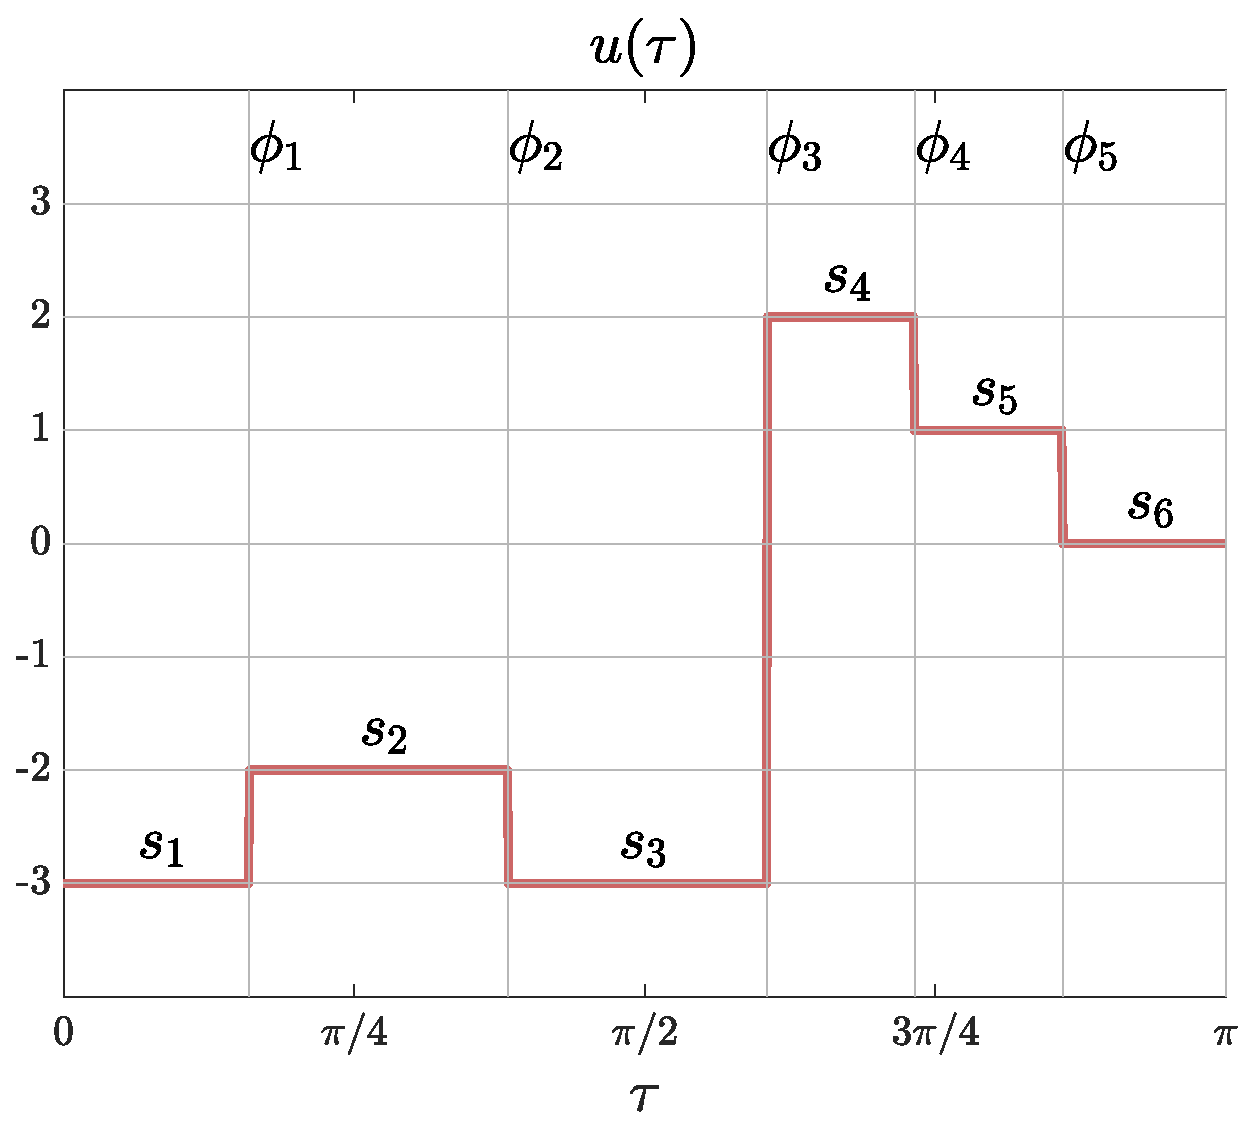
\includegraphics[scale=0.35]{img/fig01.eps} 
	\caption{A possible solution to the SHM Problem, where we considered the finite set of control $\mathcal{U} = \{-1, -1/2, 0, 1/2, 1\}$. We show the switching angles $\Phi$ and the waveform $\mS$ (see Definition \ref{def: waveform and switching angles}). The function $u(t)$ is displayed on the whole interval $[0,2\pi)$ to highlight the half-wave symmetry introduced in \eqref{eq:half-wave symmetry}.}
	\label{fig:exampleSHE}
\end{figure}

In the practical engineering applications that motivated our study, due to technical limitations, it is preferable to employ signals taking consecutive values in $\mathcal{U}$. In the sequel, we will refer to this property of the waveform as the \emph{staircase property}. We can rigorously formulate this property as follows: we say that a signal $u$ of the form \eqref{eq:uExpl} fulfills the staircase property if its waveform $\mS$ satisfies
\begin{gather}\label{eq:staircase prop}
	(s_m^{min},s_{m}^{max}) \cap \mathcal{U} = \emptyset, \quad \forall m\in \{ 0, \ldots, M-1 \},
\end{gather}
where 
\begin{align*}
	&s^{min}_m = \min\{s_m,s_{m+1}\} 
	\\[5pt]
	&s^{max}_m = \max\{s_m,s_{m+1}\}.
\end{align*}
Note that when $\mathcal{U} = \{-1,1\}$ (which is known in the SHM literature as the bi-level problem), this property is satisfied for any $u$ of the form \eqref{eq:uExpl}.

We can now formulate the SHM problem as follows:

\bigskip

\begin{problem}[SHM]\label{pb:SHEp}
Let $\mathcal{U}$ be given as in \eqref{eq:Udef}, and let $\mathcal{E} _a $ and $\mathcal{E} _b $ be two finite sets of odd numbers of cardinality $|\mathcal{E}_a| = N_a $ and $ |\mathcal{E} _b| = N_b$ respectively. For any two given vectors $\aT \in \mathbb{R}^{N_a}$ and $\bT \in \mathbb{R}^{N_b} $, construct a function $u: [0,\pi)\to\mathcal{U}$ of the form \eqref{eq:uExpl}, satisfying \eqref{eq:staircase prop}, such that the vectors $\bm{a} \in \mathbb{R}^{N_a}$ and $\bm{b} \in \mathbb{R}^{N_b}$, defined as
\begin{align}\label{vectors a and b}
	\bm{a} = \big( a_j \big)_{j\in \mathcal{E}_a} \qquad \text{and} \qquad
	\bm{b} = \big( b_j \big)_{j\in \mathcal{E}_b}
\end{align}
satisfy
\begin{align*} 
	\bm{a} = \aT \qquad \text{and} \qquad \bm{b} = \bT,
\end{align*}
where the coefficients $a_j$ and $b_j$ in \eqref{vectors a and b} are given by \eqref{eq:an}.
\end{problem}  
\vspace{1em}

\begin{remark}[SHE]\label{remark:SHE}
In Problem \ref{pb:SHEp}, we gave a very general formulation of SHM. This formulation contains also the so-called \emph{Selective Harmonic Elimination (SHE)} problem (see \cite{Sun1996}), in which the target vectors are such that 
\begin{gather}
	\notag (a_T)_1 \neq 0  \hspace{1em} (a_T)_{i\neq1} = 0 \hspace{1em} \forall i \in \mathcal{E}_a 
	\\[3pt]
	\notag (b_T)_1 \neq 0  \hspace{1em} (b_T)_{j\neq1} = 0 \hspace{1em} \forall j \in \mathcal{E}_b. 
\end{gather}
SHE is of great relevance in the electric engineering literature. Its objective is to generate a signal with amplitude $m_1 = \sqrt{a_1^2+b_1^2}$ and phase $\varphi_1=\arctan(b_1/a_1)$, removing the high-frequency components. In this way, SHE may be understood as a generator of clean Fourier modes through a staircase signal.
\end{remark}

\section{SHM as a finite-dimensional optimization problem}\label{sec:SHE_finite-dim_pbm}

A typical approach to address the SHM Problem \ref{pb:SHEp} (\cite{Yang2015,Konstantinou2010,Sun1996}) consists in looking for solutions having a specific waveform determined a priori and finding the suitable switching angles $\Phi$ allowing to reach the desired target. 

Note that, for a fixed waveform $\mS$, the Fourier coefficients of a function $u$ of the form \eqref{eq:uExpl} can be written in terms of the switching angles $\Phi$ in the following way:
\begin{align*}
	& a_j = a_j(\Phi) =  \frac{2}{j\pi} \sum_{m=0}^{M} s_m \Big[\sin(j\phi_{m+1}) -\sin(j\phi_{m})\Big]
	\\[5pt]
	& b_j = b_j(\Phi) = \frac{2}{j\pi} \sum_{m=0}^{M} s_m \Big[\cos(j\phi_{m}) -\cos(j\phi_{m+1})\Big]
\end{align*}
Hence, for two sets of odd numbers $\mathcal{E}_a$ and $\mathcal{E}_b$ as in Problem \ref{pb:SHEp}, and any fixed waveform $\mS$, we can define the functions
\begin{align*}
	&\bm{a}_\mS (\Phi) := \big(a_j (\Phi)\big)_{j\in \mathcal{E}_a} \in \mathbb{R}^{N_a}
	\\
	&\bm{b}_\mS (\Phi) := \big(b_j (\Phi)\big)_{j\in \mathcal{E}_b} \in \mathbb{R}^{N_b}
\end{align*}
and SHM can be cast as a finite-dimensional optimization process consisting in minimizing, over the choice of $\Phi = \{\phi_m\}_{m=1}^{M}$, the euclidean distance between the vectors $(\bm{a},\bm{b})$ and $(\aT,\bT)$ as defined in Problem \ref{pb:SHEp}.

\bigskip

\begin{problem}[Optimization problem for SHM]\label{pb:SHE opt}
Let $\mathcal{E}_a$, $\mathcal{E}_b$ and the targets $\aT$ and $\bT$ be given as in Problem \ref{pb:SHEp}.  Let $\mathcal S := \{ s_m\}_{m=0}^M$ be a fixed waveform satisfying \eqref{eq:staircase prop}.  Find the switching angles $\Phi$ solution to the following minimization problem:
\begin{align}
	&\min_{\Phi \in [0,\pi]^{M}} \Big( \|\bm{a}_\mS (\Phi) - \aT\|^2 + \| \bm{b}_\mS (\Phi) - \bT\|^2\Big)\notag 
	\\[10pt]
	&\mbox{subject to: } 0 = \phi_0 <\phi_1 < \ldots < \phi_{M} < \phi_{M+1} = \pi. \notag 
\end{align}
\end{problem}
At this regard, it is important to notice that the optimization Problem \ref{pb:SHE opt} solves the original Problem \ref{pb:SHEp} only when the optimal cost is zero. This makes necessary to fully characterize the space of targets $(\aT,\bT)$ for which there exists a solution. With this aim, we will define the the \textit{optimal cost} and the \textit{solvable set} as follows:
\vspace{1em}
\begin{definition}[optimal cost]
We call \textit{optimal cost} $V_{\mS}:\mathbb{R}^{N_a}\times \mathbb{R}^{N_b} \rightarrow \mathbb{R}$, the function that takes as input variables the target vectors $\aT$ and $\bT$ and returns the optimal cost of the Problem \ref{pb:SHE opt}.
\end{definition}

\vspace{1em}
\begin{definition}[solvable set]
We define a \textit{solvable set} $\mathcal{R}_{\mS}$ as:
\begin{gather}
	\mathcal{R}_{\mS} = \Big\{ (\aT,\bT) \in \mathbb{R}^{N_a+N_b}\;\big|\; V_{\mS}(\aT,\bT) = 0\Big\}
\end{gather}
\end{definition}
In practical applications, one is only interested in solutions of Problem \ref{pb:SHE opt} corresponding to $(\aT,\bT) \in \mathcal{R}_\mS$, so that it would be desirable to obtain a control function providing the switching angles $\Phi^*_\mS$ for the whole set $\mathcal{R}_\mS$. We will refer to this function as the \textit{policy} with waveform $\mS$.

\vspace{1em}
\begin{definition}[policy]
We will call \textit{policy} a function $\Pi_{\mS}: \mathcal{R}_\mS \rightarrow [0,\pi]^M$ such that $\Phi^* = \Pi_{\mS}(\aT,\bT)$, with $\Phi^*$ the optimal switching angles solutions of Problem \ref{pb:SHEp} for the targets $(\aT,\bT)$.
\end{definition} 

With the aim of reconstructing the policy $\Pi_{\mS}$, a typical approach is to solve numerically Problem \ref{pb:SHE opt} for a limited number of points in $\mathbb{R}^{N_a+N_b}$ and check that the optimal cost is zero. Secondly, one interpolates the function $\Pi_{\mS}$ in the convex set generated by the points previously obtained. Nevertheless, this approach has several difficulties and drawbacks.

\begin{itemize}
	\item[1.] \textit{Combinatory problem}: in practice, one does not dispose of a suitable waveform $\mS$ which yields a solution to the Problem \ref{pb:SHEp}. A common approach to solve the SHM problem consists in fixing the number of switches $M$, and then solve Problem \ref{pb:SHE opt} for  all the possible combinations of $M$ elements of $\mathcal{U}$. However, taking into account that the number of possible $M$-tuples  in $\mathcal U$ is of the order $(L-1)^M$, it is evident that the complexity of the above approach increases rapidly when $L>1$. This problem has been studied in \cite{Yang2015} where, through appropriate algebraic transformations, the authors are able to convert the SHM problem into a polynomial system whose solutions' set contains all the possible waveforms $\mathcal S$ of $M$ elements in $\mathcal{U}$. As a drawback of this approach, the number of switches $M$ needs to be prefixed. However, in some cases,  determining the number of switches which is necessary to reach the desired Fourier coefficients is not a straightforward task.
	
	\item[2.] \textit{Solvable set problem}: given a waveform $\mS$, the corresponding solvable set $\mathcal{R}_{\mS}$ is usually very small, yielding to policies $\Pi_{\mS}$ which are not very effective. This issue is typically addressed by solving Problem \ref{pb:SHE opt} for a set of waveforms $\{\mS_l\}_{l=1}^r$ and obtaining different policies $\{\Pi_{\mS_l}\}_{l=1}^r$ and solvable sets $\{\mathcal{R}_{\mS_l}\}_{l=1}^r$ for each one of them. By gathering them, one then creates a new policy which is applicable in a wider scenario. Nevertheless, due to the fact that in general to different waveforms may correspond disjoint or even overlapping solvable sets, this union of policies is chaotic, providing different solutions for the same target vector $(\aT,\bT)$, or even generating regions with no solution (see Fig. \ref{fig:chaos_policy}).
	
	\begin{figure}[h]
		\centering
		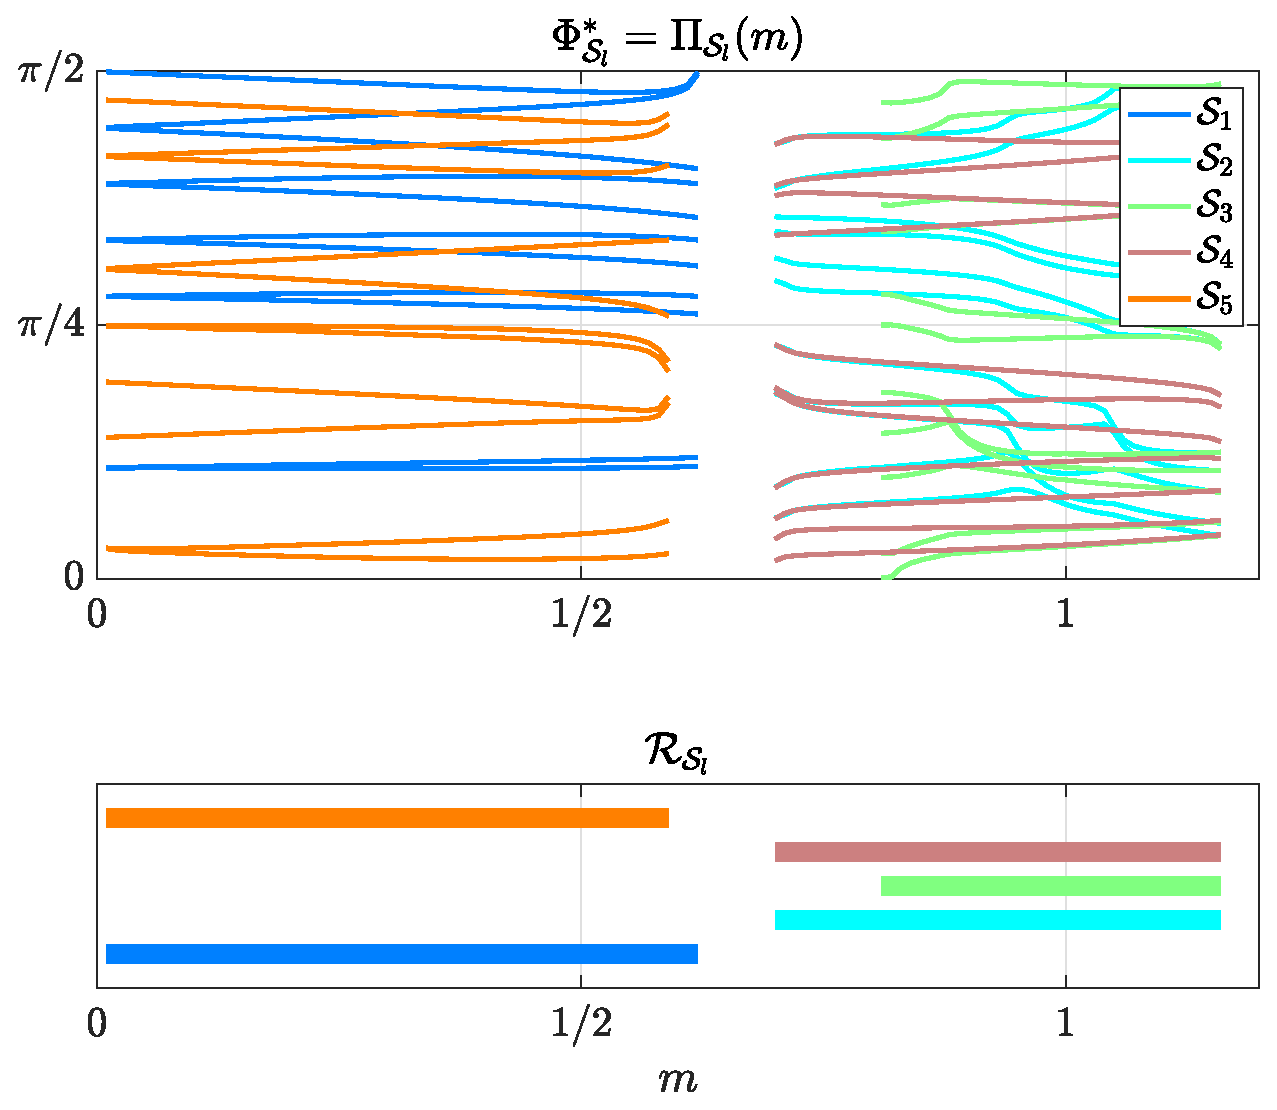
\includegraphics[scale=0.34]{img/fig01a.eps}
		\caption{In the first picture, we display the optimal switching angles $\Phi^*_{\mS}$ associated to different waveforms $\{\mS_l\}_{l=1}^7$ for a SHE problem (see Remark \ref{remark:SHE}), considering the sets $\mathcal{E}_a = \{1\}$ and $\mathcal{E}_b = \{1,5,7,11,13,17,19,23,25,29,31\}$. We chose the target $(a_1,b_1) = (m,0) \hspace{0.5em} \forall m \in [0,1.2]$. The second figure shows the solvable sets for each waveform we considered.}
		\label{fig:chaos_policy}
	\end{figure}

	\item[3.] \textit{Policy problem}: due to the complexity of a policy generated by uniting different waveforms, the continuity of the switching angles cannot be guaranteed. This is a well known problem in the SHM community \cite{Agelidis2008,Dahidah2008,Dahidah2015,Yang2017} (see Fig. \ref{fig:chaos_policy}).	
\end{itemize}

%\subsection{Combinatory problem}\label{subsec:Combinatory Problem}
%In practice, one does not dispose of a suitable waveform $\mS$ which yields a solution to the Problem \ref{pb:SHEp}. A common approach to solve the SHM problem consists in fixing the number of switches $M$, and then solve Problem \ref{pb:SHE opt} for  all the possible combinations of $M$ elements of $\mathcal{U}$. However, taking into account that the number of possible $M$-tuples  in $\mathcal U$ is of the order $(L-1)^M$, it is evident that the complexity of the above approach increases rapidly when $L>1$. This problem has been studied in \cite{Yang2015} where, through appropriate algebraic transformations, the authors are able to convert the SHM problem into a polynomial system whose solutions' set contains all the possible waveforms $\mathcal S$ of $M$ elements in $\mathcal{U}$. As a drawback of this approach, the number of switches $M$ needs to be prefixed. However, in some cases,  determining the number of switches which is necessary to reach the desired Fourier coefficients is not a straightforward task.
%
%\subsection{Solvable set problem}\label{subsec: resolvable set probem }
%
%Given a waveform $\mS$, the corresponding solvable set $\mathcal{R}_{\mS}$ is usually very small, yielding to policies $\Pi_{\mS}$ which are not very effective. This issue is typically addressed by solving Problem \ref{pb:SHE opt} for a set of waveforms $\{\mS_l\}_{l=1}^r$ and obtaining different policies $\{\Pi_{\mS_l}\}_{l=1}^r$ and solvable sets $\{\mathcal{R}_{\mS_l}\}_{l=1}^r$ for each one of them. By gathering them, on then creates a new policy which is applicable in a wider scenario. Nevertheless, due to the fact that in general to different waveforms may correspond disjoint or even overlapping solvable sets, this union of policies is chaotic, providing different solutions for the same target vector $(\aT,\bT)$, or even generating regions with no solution (see Figure \ref{fig:chaos_policy}).
%
%\begin{figure}[h]
%	\centering
%	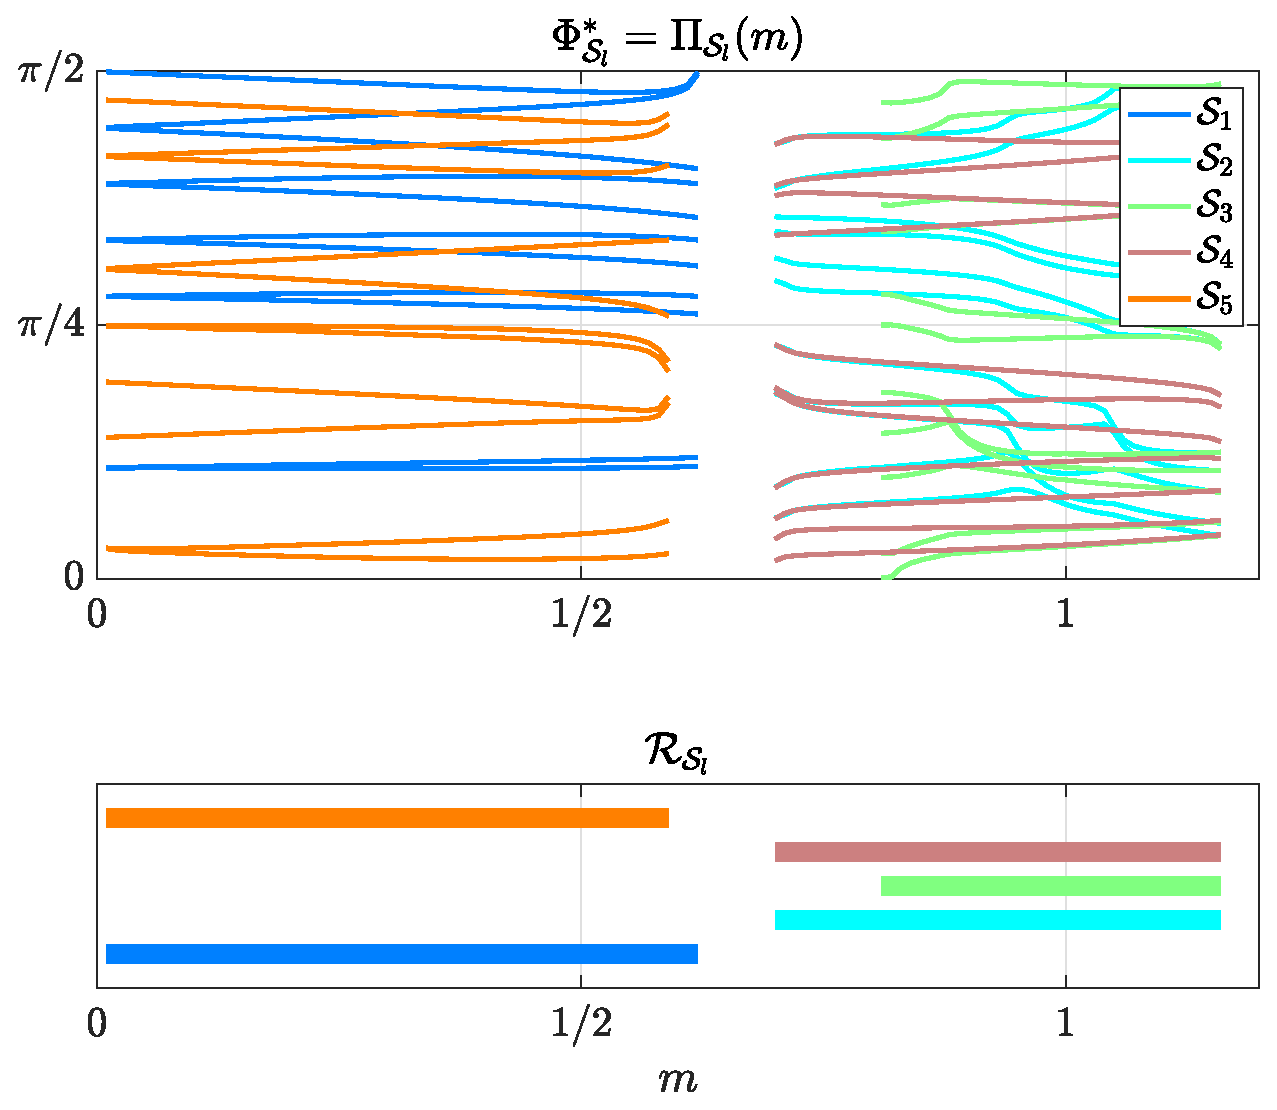
\includegraphics[scale=0.35]{img/fig01a.eps}
%	\caption{In the first picture, we display the optimal switching angles $\Phi^*_{\mS}$ associated to different waveforms $\{\mS_l\}_{l=1}^7$ for a SHE problem (see Remark \ref{remark:SHE}), considering the sets $\mathcal{E}_a = \{1\}$ and $\mathcal{E}_b = \{1,5,7,11,13,17,19,23,25,29,31\}$. We chose the target $(a_1,b_1) = (m,0) \hspace{0.5em} \forall m \in [0,1.2]$. The second figure shows the solvable sets for each waveform we considered.}
%	\label{fig:chaos_policy}
%\end{figure}
%
%\subsection{Policy problem} \label{subsec:Non-continuous policy}
% 
%Due to the complexity of a policy generated by the union of different waveforms, the continuity of the switching angles cannot be guaranteed. This is a well known problem in the SHM community \cite{Agelidis2008,Dahidah2008,Dahidah2015,Yang2017} (see Figure \ref{fig:chaos_policy}).
As we shall see, all these mentioned criticalities will be overcome by our optimal control approach.

\section{SHM as an optimal control problem}\label{sec:Contributions}

Our main contribution in the present paper consists in formulating the SHM problem from the viewpoint of optimal control. In this formulation, the Fourier coefficients of the signal $u(t)$ are identified with the terminal state of a controlled dynamical system of $N_a+N_b$ components defined in the time-interval $[0,\pi)$.  The control of the system is precisely the signal $u(t)$, defined as a function from $[0,\pi)$ to $\mathcal{U}$, which has to steer the state from the origin to the desired values of the prescribed Fourier coefficients. 

The starting point of this approach is to rewrite the Fourier coefficients of the function $u(t)$ as the final state of a dynamical system controlled by $u(t)$. To this end, let us first note that, in view of \eqref{eq:an}, for all $u\in L^\infty ([0,\pi);\mathbb{R})$ any Fourier coefficient $a_j$ satisfies
\begin{align*}
	a_j = y(\pi), 
\end{align*}
with $y\in C([0,\pi);\mathbb{R})$ defined as
\begin{align*}
	y(t) = \dfrac{2}{\pi} \int_0^t u(\tau) \cos(j\, \tau) d\tau.
\end{align*}
Besides, as a consequence of the fundamental theorem of calculus, $y(\cdot)$ is the unique solution to the differential equation
\begin{equation}\label{eq: ODE Fourier}
	\begin{cases}
		\dot{y} (t) = \dfrac{2}{\pi} \cos(j\, t) u(t), \qquad  t\in [0,\pi)
		\\[5pt]
		y(0) = 0.
	\end{cases}
\end{equation}
Analogously, we can also write the Fourier coefficients $b_j$, defined in \eqref{eq:an}, as the solution at time $t=\pi$ of a differential equation similar to \eqref{eq: ODE Fourier}.

Hence, for $\mathcal{E}_a$, $\mathcal{E}_b$, $\aT$ and $\bT$ given, the SHM Problem \ref{pb:SHEp} can be reduced to finding a control function $u$ of the form \eqref{eq:uExpl}, satisfying \eqref{eq:staircase prop}, such that the corresponding solution $\bm{y} \in C([0,\pi]; \mathbb{R}^{N_a+N_b})$ to the dynamical system
\begin{equation}\label{eq:forward dyn syst}
	\begin{cases}
		\dot{\bm{y}}(t) = \dfrac{2}{\pi} \bm{\mathcal{D}}(t) u(t), \qquad  t\in [0,\pi)
		\\[5pt]
		\bm{y}(0) = 0.
	\end{cases}
\end{equation}
satisfies
\begin{align*}
	\bm{y} (\pi) = [\aT;\bT]^\top,	
\end{align*}
where
\begin{equation}\label{eq:Dynamics}
	\bm{\mathcal{D}}(t) = \left[ \bm{\mathcal{D}}^a(t); \bm{\mathcal{D}}^b(t) \right]^\top, 
\end{equation}
with $\bm{\mathcal{D}}^a(t) \in \mathbb{R}^{N_a} $ and $ \bm{\mathcal{D}}^b(t) \in \mathbb{R}^{N_b}$ given by
\begin{gather}\label{eq:DalphaDbeta}
    \begin{align}
        \bm{\mathcal{D}}^a(t) = 
        \begin{bmatrix} 
            \cos(e_a^1t) \\ \cos(e_a^2t) \\ \vdots \\ \cos(e_a^{N_a}t) 
        \end{bmatrix},
        \quad \bm{\mathcal{D}}^b(t) = 
        \begin{bmatrix} 
            \sin(e_b^1t) \\ \sin(e_b^2t) \\ \vdots \\ \sin(e_b^{N_b}t)
        \end{bmatrix} 
    \end{align} 
\end{gather}
Here, $e_a^i$ and $e_b^i$  denote the elements in $\mathcal{E}_a$ and  $\mathcal{E}_b$, i.e.
\begin{align*}
	\mathcal{E}_a = \{e_a^1,e_a^2,e_a^3,\dots,e_a^{N_a}\}, \quad \mathcal{E}_b = \{e_b^1,e_b^2,e_b^3,\dots,e_b^{N_b}\}.
\end{align*}
Moreover,for notation simplicity, we reverse the time in \eqref{eq:forward dyn syst} using the transformation $\bm{x} (t) = \bm{y}(\pi - t)$. In this way, the SHM problem converts into the following null controllability one for a dynamical system with initial condition $\bm{x}(0) = [\aT; \bT]^\top$ (see also Fig. \ref{fig:evolution_x}).

\medskip

\begin{problem}[SHM via null controllability]\label{pb:SHEpControl}
Let $\mathcal{U}$ be given as in \eqref{eq:Udef}, and let $\mathcal{E}_a $ and $\mathcal{E}_b $ be two finite sets of odd numbers of cardinality $|\mathcal{E}_a| = N_a $ and $ |\mathcal{E}_b| = N_b$, respectively. For any two given vectors $\aT \in \mathbb{R}^{N_a}$ and $\bT \in \mathbb{R}^{N_b} $,  we look for a function $u: [0,\pi)\to [-1,1]$ of the form \eqref{eq:uExpl}, satisfying \eqref{eq:staircase prop}, such that the solution to the initial-value problem
\begin{equation}\label{eq:CauchyReversed}
	\begin{cases}
        \displaystyle\dot{\bm{x}}(t) = -\frac 2\pi\bm{\mathcal{D}}(t)u(t),  & t \in [0,\pi)
        \\[5pt]
        \bm{x}(0) = \bm{x}_0 := [\aT; \bT]
    \end{cases}
\end{equation}
satisfies $\bm{x} (\pi) = 0$, where $\bm{\mathcal{D}}$ is given by \eqref{eq:Dynamics}--\eqref{eq:DalphaDbeta}.
\end{problem}

\begin{figure}[ht!] 
    \centering
    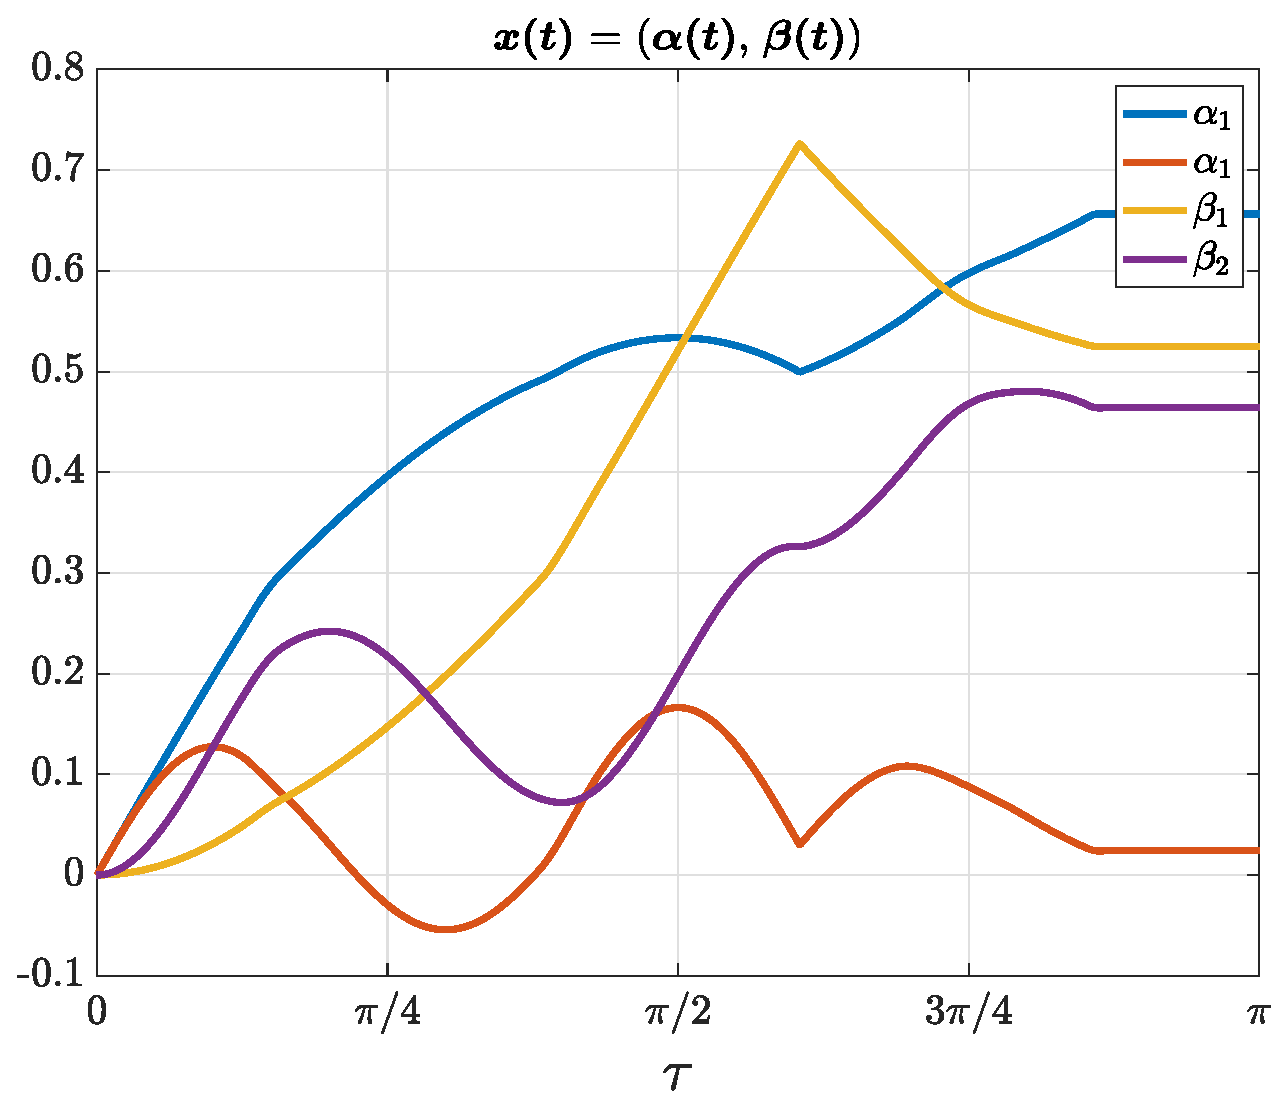
\includegraphics[scale=0.325]{img/fig02.eps}
    \caption{Evolution of the dynamical system \eqref{eq:CauchyReversed} with $\mathcal{E}_a = \{1,2\}$ and $\mathcal{E}_b = \{1,2\}$ corresponding to the control $u$ in Figure \ref{fig:exampleSHE}. The positions of the switching angles $\bm{\phi}$ are displayed as well.}\label{fig:evolution_x}
\end{figure}

A natural approach for controllability problems such as Problem \ref{pb:SHEpControl} is to formulate them as optimal control ones, where the cost functional to be minimized is the euclidean distance from the final state $\bm{x}(\pi)$ to the target, in this case, the origin. In what follows, for a given vector $\bm{v}\in\mathbb{R}^d$, we shall always denote by $\|\bm{v}\|$ the euclidean norm $\|\bm{v}\|_{\mathbb{R}^d}$. Moreover, we will denote
\begin{align*}
	&\mathcal A:= \Big\{u:[0,\pi)\to [-1,1]\; \text{ measurable}\Big\}
	\\
	&\mathcal A_{ad}:= \Big\{u\in\mathcal A \text{ of the form } \eqref{eq:uExpl} \text{ satisfying } \eqref{eq:staircase prop}\Big\}
\end{align*}


\begin{problem}[OCP for SHM]\label{pb:OCP1}
Let $\mathcal{U}$ be a given set as in \eqref{eq:Udef} and let $\mathcal{E}_a $ and $\mathcal{E} _b $ be two finite sets of odd numbers of cardinality $|\mathcal{E}_a| = N_a $ and $ |\mathcal{E} _b| = N_b$ respectively. For any two given vectors $\aT \in \mathbb{R}^{N_a}$ and $\bT \in \mathbb{R}^{N_b} $, we look for an admissible control $u\in \mathcal{A}_{ad}$ solution to the following optimal control problem:
\begin{equation*}
	\min_{u \in \mathcal{A}_{ad}}\;\frac 12 \|\bm{x}(\pi)\|^2 \quad \text{subject to the dynamics \eqref{eq:CauchyReversed}}.
\end{equation*}
\end{problem}

\begin{remark}
Note that the cost functional in Problem \ref{pb:OCP1} is quadratic and, therefore, it always admits at least one minimizer for any target $[\aT;\bT]^\top$. Nevertheless, this minimizer provides a solution of the SHM problem if and only if the corresponding minimum is equal to zero. Otherwise, we say that the target $[\aT;\bT]^\top$ is unreachable. In this work, we will not discuss the reachable set for the control problem \eqref{pb:OCP1}.
\end{remark}

A main feature of the SHM problem is that we are looking for signal functions $u$ of the form \eqref{eq:uExpl} satisfying \eqref{eq:staircase prop}. In principle, this can be guaranteed by by adding directly this constraint on the set of admissible controls $\mathcal{A}_{ad}$, as we did in Problem \ref{pb:OCP1}. Notwithstanding that, the inclusion of such a constraint makes the optimal control problem extremely difficult, as it prevents us from applying standard arguments such as the Pontryagin maximum principle, and implementing all the computational techniques developed in the last decades to solve optimal control problems. As a matter of fact, the classical tools in optimal control theory seem not to be adapted to handle such constraints on the control. 

In order to bypass this difficulty, we propose a modification of Problem \ref{pb:OCP1} by adding to the cost functional a penalization term for the control. 

\bigskip

\begin{problem}[Penalized OCP for SHM]\label{pb:OCP_penalizado}
Fix $\varepsilon>0$ and a function $\mathcal{L}\in C([-1,1];\mathbb{R})$.  Let $\mathcal{E} _a $ and $\mathcal{E} _b $ be two finite sets of odd numbers of cardinality $|\mathcal{E}_a| = N_a $ and $ |\mathcal{E} _b| = N_b$, respectively. For any two given target vectors $\aT \in \mathbb{R}^{N_a}$ and $\bT \in \mathbb{R}^{N_b} $, we look for a control $u\in \mathcal A$ solution to the following optimal control problem:
\begin{align*}
	&\displaystyle\min_{u \in \mathcal A}\;\left(\dfrac{1}{2} \|\bm{x}(\pi)\|^2 + \varepsilon \displaystyle\int_0^\pi \mathcal{L}(u(t)) dt\right) 
	\\[5pt] 
	&\text{subject to the dynamics \eqref{eq:CauchyReversed}}.
\end{align*}
\end{problem}
Observe that, in Problem \ref{pb:OCP_penalizado}, we do not impose the constraint that the control has to be the form \eqref{eq:uExpl} and satisfy the staircase property \eqref{eq:staircase prop}. Nevertheless, as we shall see, these features of $u$ will arise naturally from a suitable choice of the Lagrangian $\mathcal{L}$.

Another important aspect that needs to be taken into account is that the penalization term for the control might prevent the optimal trajectory from reaching the target. In other words, even if there exists a control for which the optimal trajectory satisfies $\bm{x} (\pi) = 0$, the optimal control in Problem \ref{pb:OCP_penalizado} might not do so, and therefore, the solution to Problem \ref{pb:OCP_penalizado} would not be a solution to the SHM problem. This issue may be prevented by a proper selection of the weighting parameter $\varepsilon$ which allows to tune the precision of the optimal control for the perturbed problem, guaranteeing that the final state of the optimal trajectory is close enough to zero. In more detail, we have the following result.

\bigskip

\begin{proposition}\label{Prop:approx controllability}
Assume that $[\aT,\bT]^\top$ is such that Problem \ref{pb:SHEpControl} admits a solution, and let $u^\ast\in \mathcal A$ be the solution to Problem \ref{pb:OCP_penalizado}. Then the associated trajectory $\bm{x}^\ast\in C([0,\pi);\mathbb{R})$, solution to \eqref{eq:CauchyReversed}, satisfies
\begin{align*} 
	\| \bm{x}^\ast (\pi)  \|^2 \leq  4 \varepsilon \pi \| \mathcal{L}\|_\infty,
\end{align*}
where $\| \cdot\|_\infty$ denotes the max-norm in $C([-1,1]; \mathbb{R})$.
\end{proposition}

The proof of Proposition \ref{Prop:approx controllability} is postponed to Section \ref{sec:Proof}. Let us now describe the construction of penalization functions $\mathcal{L}$ which guarantee that any solution to Problem \ref{pb:OCP_penalizado} has the form \eqref{eq:uExpl} and satisfies \eqref{eq:staircase prop}. To this end, we will distinguish two cases, depending on the cardinality of $\mathcal{U}$.

\subsection{Bilevel SHM problem via OCP (Bang-Bang Control)} 

In this case, the control set $\mathcal{U}$ defined in \eqref{eq:Udef} has only two elements, i.e.  $\mathcal{U}=\{-1,1\}$.
In the control theory literature, a control taking only two values is known as \emph{bang-bang control}. In the SHM literature, this kind of solution are called \textit{bi-level solutions}. Note that in this case, any $u$ with the form \eqref{eq:uExpl}  trivially satisfies the staircase property \eqref{eq:staircase prop}.

The first main result of the present paper is the following.

\bigskip
\begin{theorem}\label{th:bang-bang}
Let $\mathcal{U}=\{ -1, 1\}$, and consider Problem \ref{pb:OCP_penalizado}. If the function $\mathcal{L}\in C([-1,1];\mathbb{R})$ is concave, then any optimal control $u^\ast$, solution to Problem \ref{pb:OCP_penalizado}, has a bang-bang structure, i.e. it has the form \eqref{eq:uExpl}.
\end{theorem}

The proof of Theorem \ref{th:bang-bang} is postponed to Section \ref{sec:Proof}, and follows from the optimality conditions given by the Pontryagin's maximum principle. In particular, the fact that the control $u$ acts linearly in \eqref{eq:CauchyReversed}, together with the concavity of $\mathcal{L}$, implies that the Hamiltonian is also concave, and then, the minimum is always attained at the limits of the interval $[-1,1]$.

We point out that, by choosing different penalization functions $\mathcal{L}$, we can obtain solutions to the SHE problem with different waveforms.
Typical choices which give rise to bang-bang controls are 
\begin{align*}
	\mathcal{L}(u) = u,  \quad \mathcal{L}(u) = -u,  \quad \mathcal{L}(u) = -u^2.
\end{align*} 
See Fig. \ref{fig:Bang-Bang-penalization} for an illustration.

\subsection{Multilevel SHM problem via OCP}

Inspired by the ideas of the previous subsection, we can address the case when $\mathcal{U}$ contains more than two elements. This is known in the power electronics literature as the \textit{multilevel SHM problem}. Now, the goal is to construct a function $\mathcal{L}$ such that the Hamiltonian associated to Problem \ref{pb:OCP_penalizado} always attains the minimum at points in $\mathcal{U}$.
A way to construct such a function $\mathcal{L}$ is to interpolate a parabola in $[-1,1]$ by affine functions, considering the elements in $\mathcal{U}$ as the interpolating points.  Since, between any two points in $\mathcal{U}$,  the function $\mathcal{L}$ is a straight line,  the Hamiltonian is a concave function in these intervals, and hence, the minimum is always attained at points in $\mathcal{U}$.

\vspace{1em}
\begin{theorem}\label{th:PLP}
Let $\mathcal{U}$ be a given set as in \eqref{eq:Udef}. For some $0<a\in\mathbb{R}$ and $b\in \mathbb{R}$, set the function
\begin{align}\label{eq:parabola}
	\mathcal{P}(u) = a (u-b)^2.
\end{align}
Consider Problem \ref{pb:OCP_penalizado} with 
\begin{align}\label{eq:PLP}
	&\mathcal{L}(u) = \begin{cases}
            \lambda_k(u) & \text{if }  u \in [u_k,u_{k+1}) \\ \mathcal{P}(1) & \text{if } u = u_{L} 
    \end{cases} 
	\\[10pt]
	&\notag \forall k \in \{1,\dots,L-1\}, 
\end{align}
where 
\begin{align}\label{eq:lambda k}
	\lambda_k(u):= \dfrac{ (u-u_k)\mathcal{P}(u_{k+1}) + (u_{k+1}- u) \mathcal{P}(u_k)}{u_{k+1} - u_k}.
\end{align}
Then any optimal control $u^\ast$, solution to Problem \ref{pb:OCP_penalizado}, has the form \eqref{eq:uExpl} and satisfies \eqref{eq:staircase prop}.
\end{theorem}

\medskip

\begin{remark}
For completeness, we shall mention that in Theorem \ref{th:PLP} the Lagrangian $\mathcal L$ can actually have a more general form, still yielding to a staircase optimal control $u^\ast$. As a matter of fact, as we shall see in Section \ref{sec:Proof}, the proof of Theorem \ref{th:PLP} does not use the fact that the function $\mathcal P$ is a parabola. If we replace this $\mathcal P$ with any other strictly convex function (such as a polynomial of even degree), our result remains valid. The choice we made of defining $\mathcal P$ as in \eqref{eq:parabola} is motivated by the fact that, most often, in optimal control theory the penalization terms are chosen to be quadratic.
\end{remark}

\medskip

\begin{remark}[\emph{Bang-off-bang control}]
We note that when  $\mathcal{U}= \{-1,0,1\}$, we can just use the $L^1$-norm of the control as penalization, i.e. $\mathcal{L}(u) = |u|$. This yields to the so-called \emph{bang-off-bang} controls, that are widely studied in the literature \cite{nagahara2013maximum,ikeda2016maximum}. By taking a different parabola $\mathcal{P}$, one can then obtain different bang-off-bang solutions to the SHM problem.
\end{remark}

We illustrate in Fig. \ref{fig:SHE-multi} different examples of penalization functions $\mathcal{L}$ giving rise to multilevel solutions to the SHM problem. We point out that, by varying the values of $a$ and $b$ in Theorem \ref{th:PLP}, we can obtain solutions with different waveforms.

\bigskip

\section{Numerical simulations}\label{sec:Simulations}

In this section, we present several examples in which we implement the optimal control strategy we proposed to solve the SHM problem. All the simulations we are going to present can be found also in \cite{simus}. Our Experiments were conducted on a personal MacBook Pro laptop (1,4 GHz Quad-Core Intel Core i5, 8GB RAM, Intel Iris Plus Graphics 1536 MB). 

To solve our optimal control Problem \ref{pb:OCP_penalizado}, we will employ the direct method \cite{rao2009survey} which, in broad terms, consists in discretizing the cost functional and the dynamics, and then apply some optimization algorithm. 

The dynamics will be approximated with the \UB{Runge-Kutta 6} method, while for solving the discrete minimization problem we will employ the non-linear constrained optimization tool \texttt{CasADi} \cite{Andersson2019}. \texttt{CasADi} is an open-source tool for nonlinear optimization and algorithmic differentiation which implements the interior point method. To be efficiently applied to solve an optimal control problem, we then need the functional we aim to minimize to be smooth. This is not the case of the functional in Problem \ref{pb:OCP_penalizado} which, due to the piece-wise linear penalization, is not differentiable at the points $u_k\in\mathcal U$. For this reason, we will first need to build a smooth approximation of the Lagrangian function $\mathcal L$ we introduced in \eqref{eq:PLP}. Once we have this approximation, we will employ the optimal control approach we presented in Section \ref{sec:Contributions} to solve some specific examples of SHM problem.

\subsection{Smooth approximation of piece-wise linear penalization}

As we mentioned, to efficiently employ \texttt{CasADi} for solving our optimal control problem, we need to build a smooth approximation of the cost functional. For this reason, we will regularize the piece-wise linear penalization defined in \eqref{eq:PLP} in the following way.

First of all, for all real $\theta>0$, we introduce the $C^\infty(\mathbb{R})$ function
\begin{align*}
	\displaystyle h^\theta(x) := \frac{1 + \tanh(\theta x)}{2}
\end{align*}
and observe that, as $\theta\to +\infty$, $h^\theta$ converges in $L^\infty(\mathbb{R})$ to the Heaviside function 
\begin{align*}
    h(x) = \begin{cases}
        1 & \text{ if } x > 0 
        \\
		0 & \text{ if } x \leq 0
    \end{cases}.
\end{align*}
Secondly, for all $k \in \{1,\dots,N_u-1\}$ we define the (smooth) function $\Pi_{[u_k,u_{k+1})}^\theta:\mathbb{R} \rightarrow \mathbb{R}$ given by
\begin{align*}
	\Pi_{[u_k,u_{k+1})}^\theta(x) :&= - 1 + h^\theta(x-u_k) + h^\theta(-x+u_{k+1}) 
	\\[5pt]
	&= \frac{\tanh[\theta(x-u_k)] + \tanh[\theta (u_{k+1}-x)]}{2}
\end{align*}
which, as $\theta\to +\infty$, converges in $L^\infty(\mathbb{R})$ to the characteristic function $\chi_{[u_k,u_{k+1})}$.

Finally, we employ $\Pi_{[u_k,u_{k+1})}^\theta$ to define
\begin{align}\label{eq:Lsmooth}
	\mathcal{L}^\theta(u) = \sum_{k = 1}^{N_u-1} \lambda_k \Pi^\theta_{[u_k,u_{k+1})}(u),
\end{align}
with $\lambda_k$ given by \eqref{eq:lambda k}, which, as $\theta\to +\infty$, converges in $L^\infty(\mathbb{R})$ to the penalization function $\mathcal L$ defined in \eqref{eq:PLP}.

Finally, notice that this regularization procedure is independent of the function $\lambda_k$ in \eqref{eq:PLP}, which is just required to be in the form \eqref{eq:lambda k}. Nevertheless, in our numerical experiments we shall select some specific $\lambda_k$. In particular, we will use 
\begin{gather}
	\lambda_k = (u_{k+1}+u_{k}) (u-u_k) + u_k^2, 
\end{gather}
which corresponds to taking $a=1$ and $b=0$ in \eqref{eq:parabola}.

\subsection{Direct method  for OCP-SHE}

To solve the optimal control Problem \ref{pb:OCP_penalizado}, we use a direct method, whose starting point is to discretize the cost functional and the dynamics.

To this end, let us consider a $N_t$-points partition of the interval $[0,\pi]$ 
\begin{displaymath} 
	\mathcal{T} = \{t_k\}_{k=1}^{N_t} 
\end{displaymath}
and denote by $\bm{u} \in \mathbb{R}^{N_t}$ the vector with components $u_k = u(t_k)$, $k=1,\ldots,N_t$.

Then the optimal control Problem \ref{pb:OCP1} can be written as optimization problem with variable $\bm{u} \in \mathbb{R}^{N_t}$. In particular, given a partition of the interval $[0,\pi)$, we can formulate Problem \ref{pb:OCP_penalizado} as the following one in discrete time.
\newline

\begin{problem}[Numerical OCP]\label{pb:numOCP2}
Given two sets of odd numbers $\mathcal{E}_a$ and $\mathcal{E}_b$ with cardinalities $|\mathcal{E}_a| = N_a$ and $|\mathcal{E}_b| = N_b$, respectively, the target vectors $\aT \in \mathbb{R}^{N_a}$ and $\bT \in \mathbb{R}^{N_b}$, and the partition $\mathcal{T}$ of the interval $[0,\pi]$, we look for $\bm{u} \in \mathbb{R}^{N_t}$ that solves the following minimization problem:
\begin{align*}
	&\min_{\bm{u} \in \mathbb{R}^{N_t}} \Bigg[\| \bm{x}_{N_t}\|^2 + \varepsilon \sum_{k=1}^{N_t-1} 
	\bigg[\frac{\mathcal{L}^\theta(u_{t_k}) + \mathcal{L}^\theta(u_{t_{k+1}})}{2}\Delta t_k \bigg]  \Bigg]  
	\\[15pt]
    &\notag \text{subject to: } 
    \\
    &\forall \tau \in \mathcal{P} \begin{cases}
    \bm{x}_{t_{k+1}} = \bm{x}_{t_k} - \Delta t_{k} (2/\pi) \bm{\mathcal{D}}(t_k)\\
    \bm{x}_{t_1} = \bm{x}_0:= [\aT,\bT]^\top
    \end{cases} 
\end{align*}
where 
\begin{gather}
	\Delta t_{k} = t_{k+1} - t_{k} \hspace{1em} \forall k \in \{1,\dots,N_t-1\}.
\end{gather}
\end{problem}

\subsection{Numerical experiments}

We now present several numerical experiments to show the effectiveness of our optimal control approach to solve SHM problems. All the examples that we are going to present will share the following common parameter: $\varepsilon = 10^{-5}$, $\theta = 10^5$ and $\mathcal{P}_t = \{0,0.1,0.2,\dots,\pi\}$. Moreover, we will consider $\mathcal{E}_a = \mathcal{E}_b = \{1,5,7,11,13,15\}$, and the target vectors $\aT = \bT = (m,0,0,0,0,0)^\top$ for all values of $m \in [-0.8,0.8]$. 

We will treat all the specific types of controls we mentioned before, that is
\begin{itemize}
	\item[1.] \emph{bang-bang}, with $\mathcal{U} = \{-1,1\}$.
	\vspace{0.05cm}
	\item[2.] \emph{bang-off-bang}, with $\mathcal{U} = \{-1,0,1\}$. 
	\vspace{0.05cm}
	\item[3.] \textit{multilevel}, $\mathcal{U} = \{-1,-1/2,0,1/2,1\}$.
\end{itemize}

The results of our simulations are displayed in Fig. \ref{fig:sim-bang-bang}, \ref{fig:sim-bang-off-bang} and \ref{fig:sim-multi-level}.

\begin{figure}[ht!]
    \hspace{0.05em}
    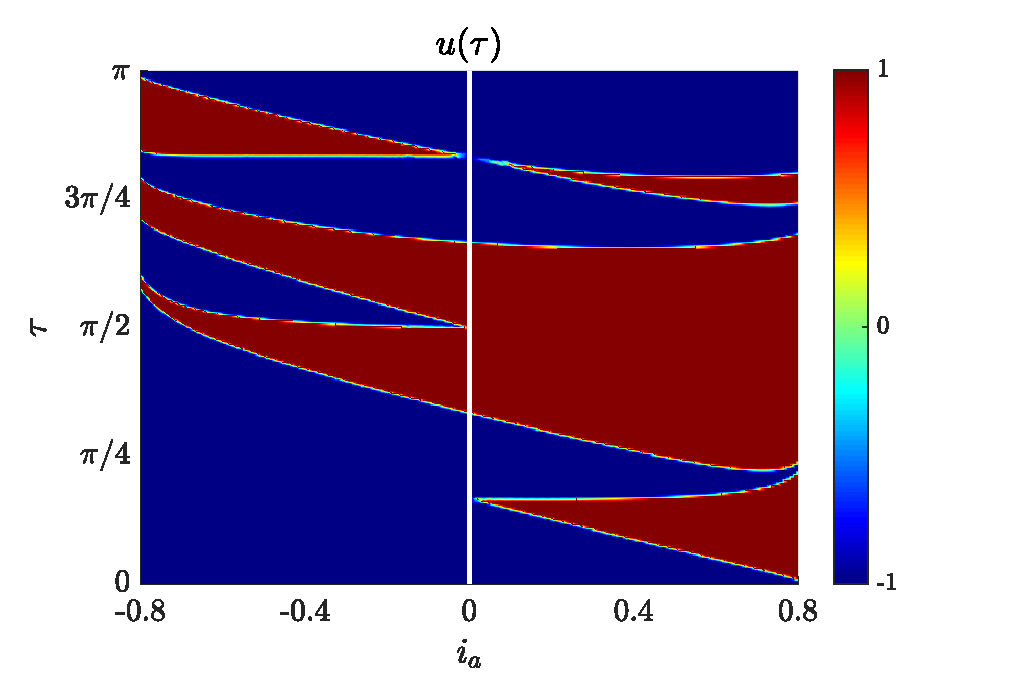
\includegraphics[scale=0.525]{img/fig05.eps}
    \caption{Bang-bang control for the SHM problem.}\label{fig:sim-bang-bang}
\end{figure} 

\begin{figure}[ht!]
    \hspace{0.05em}
    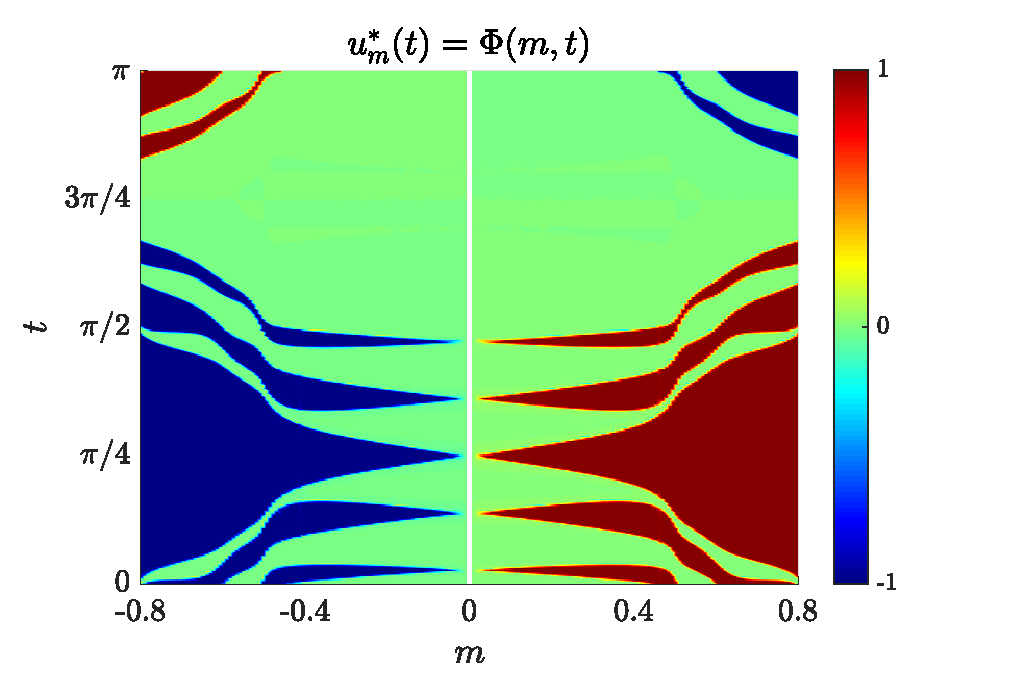
\includegraphics[scale=0.525]{img/fig06.eps}
    \caption{Bang-off-bang control for the SHM problem.}\label{fig:sim-bang-off-bang}
\end{figure} 

\begin{figure}[ht!]
    \hspace{0.05em}
    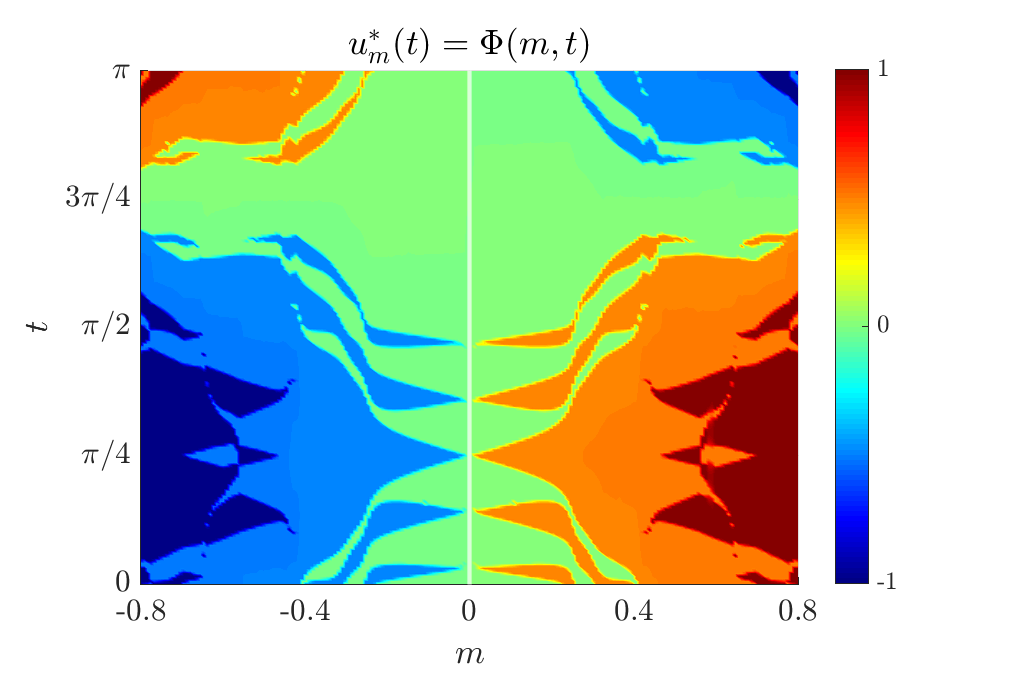
\includegraphics[scale=0.525]{img/fig08.eps}
    \caption{Multilevel control for the SHM problem.}
    \label{fig:sim-multi-level}
\end{figure} 

In these plots, to each value of the parameter $m$ in the horizontal line, it corresponds an optimal control having a staircase structure and changing value in $\mathcal U$ in the correspondence of the change of color. For instance, in Fig. \ref{fig:sim-bang-bang}, the control will be $u=-1$ in the blue region and $u=1$ in the red one.

In addition to that, we can see in all the figures that the issues we mentioned in Section \ref{sec:SHE_finite-dim_pbm} concerning the solvable set and the continuity of the policy have been overcome by our approach. This is because, while solving Problem \ref{pb:numOCP2}, we are not restricted to have a specific waveform, as it is Problem \ref{pb:SHE opt}. Instead, for any value of $m$ the best waveform and switching angles to reach the desired targets are automatically obtained through the minimization process to compute the optimal control. In other words, the possibility of changing the waveform during the optimization process can be seen as an extra degree of freedom allowing to have a large solvable set and a continuous policy. Furthermore, also the \textit{combinatory problem} we introduced in Section \ref{sec:SHE_finite-dim_pbm} is solved by our approach, as we do not need anymore to launch the same optimization process for all the possible waveforms of a given set $\mathcal U$. 

All these considerations show that the methodology introduced in this paper is theoretically and computationally competitive to solve the SHM problem.



\section{Proofs of results in Section \ref{sec:Contributions}}\label{sec:Proof}

We give here the proofs of the results presented in Section \ref{sec:Contributions}. We start with the proof of Proposition \ref{Prop:approx controllability}, which gives an upper estimate for the error in the solution to the optimal control problem with the penalization term for the control. 

\bigskip

\begin{proof}[of Proposition \ref{Prop:approx controllability}]
Since we are supposing that Problem \ref{pb:SHEpControl} has a solution, there exists a control $\tilde{u}\in L^\infty$ such that its corresponding trajectory $\tilde{\bm{x}}$, solution to \eqref{eq:CauchyReversed}, satisfies $\tilde{\bm{x}}(\pi) = 0$. 

Now, let $u^\ast$ be the solution to Problem \ref{pb:OCP_penalizado}, and let $\bm{x}^\ast$ be its corresponding trajectory. By the optimality of $u^\ast$ we have
\begin{align*}
	\frac{1}{2} \| \bm{x}^\ast(\pi)\|^2 +\varepsilon \int_0^\pi \mathcal{L}(u^\ast(\tau))d\tau \leq \varepsilon \int_0^\pi \mathcal{L}(\tilde{u}(\tau))d\tau,
\end{align*}
and hence, we deduce that $\| \bm{x}^\ast (\pi)\|^2 \leq 4 \varepsilon \pi \| \mathcal{L}\|_\infty.$ \hfill $\square$
\end{proof}

\subsection{Proofs of Theorems \ref{th:bang-bang} and \ref{th:PLP}}

The proofs of Theorems \ref{th:bang-bang} and \ref{th:bang-bang} are based on the optimality conditions for the Optimal Control Problem \ref{pb:OCP_penalizado}, which can be deduced by means of Pontryagin's maximum principle \cite[Chapter~2.7]{bryson1975applied}.

To this end, let us first introduce the Hamiltonian function associated to the Optimal Control Problem \ref{pb:OCP_penalizado}:
\begin{align}\label{eq:hamil}
    \mathcal{H}(u,\bm{p},t) = \varepsilon \mathcal{L}(u) - \frac 2\pi\big(\bm{p} \cdot \bm{\mathcal{D}}(t)\big)u(t),
\end{align}
where $\bm{p}\in \mathbb{R}^{N_a+N_b}$ is the so-called adjoint variable, which arises from the restriction imposed by the dynamical system \eqref{eq:CauchyReversed}. In view of the definition of $\bm{\mathcal{D}}(t)$ in \eqref{eq:Dynamics}-\eqref{eq:DalphaDbeta}, we will sometimes write the state and the adjoint variables using the following notation:
\begin{align*}
  \bm{x}(t) = \begin{bmatrix} \bm{a}(t) \\ \bm{b}(t) \end{bmatrix} \quad \text{and}\quad
  \bm{p}(t) = \begin{bmatrix} \bm{p}^a(t) \\ \bm{p}^b(t) \end{bmatrix}.
\end{align*}

Now, let us derive the optimality conditions arising from Pontryagin's principle.
\begin{itemize}
	\item[1.] \textbf{The adjoint system}: for any $u^\ast \in L^\infty$, solution to the Problem \ref{pb:OCP_penalizado}, there exists a unique adjoint trajectory $\bm{p}^\ast\in C([0,\pi]; \mathbb{R}^{N_a+N_b})$ which satisfies the following terminal-value problem
    \begin{equation*}
    	\begin{cases}
    		\dot{\bm{p}^\ast}(t) = -\nabla_x \mathcal{H}(u(t),\bm{p}^\ast(t),t), \qquad t \in [0,\pi] 
    		\\[5pt]
    		\bm{p}^\ast (\pi) = \nabla_x \Psi (\bm{x}^\ast (\pi))
    	\end{cases}
    \end{equation*}
    where $\Psi$ is the terminal cost of the Optimal Control Problem \ref{pb:OCP_penalizado}. In our case, we have $\Psi (\bm{x}) = \frac{1}{2} \| \bm{x}\|^2$. Moreover, since the Hamiltonian does not depend on the state variable $\bm{x}$, we simply have $\dot{\bm{p}^\ast}(t) = 0$ for all $t \in [0,\pi]$. We therefore deduce that the adjoint trajectory is constant, and given by
    \begin{equation}\label{eq:adjoint constant}
		\bm{p}^\ast (t) = \bm{x}^\ast (\pi), \qquad \forall t \in [0,\pi]. 
	\end{equation}
    
    \item[2.] \textbf{The Optimal  Control}: now, using the optimal adjoint trajectory, we can deduce the necessary optimality condition for the control, which reads as follows:
    \begin{align}\label{eq:control design}
    	u^* (t) \in \argmin_{|u|\leq 1} \mathcal{H}(t,\bm{p}^*(t),u), \quad \forall t \in [0,\pi].
    \end{align}
    As we will see, for penalization functions $\mathcal{L}$ as the ones we consider in Theorems \ref{th:bang-bang} and \ref{th:PLP}, this argmin is a singleton for almost every $t\in [0,\pi]$. Hence, given the adjoint $\bm{p}^\ast$,  condition \eqref{eq:control design} uniquely determines the control as a function in $L^\infty$.
\end{itemize}
Let us denote 
\begin{align}\label{eq:m ast}
	\mu^\ast (t) := & \frac 2\pi \big(\bm{x}^*(\pi) \cdot \bm{\mathcal{D}}(t)\big) 
	\\[5pt]
	= & \sum_{i \in \mathcal{E}_a} a^*_i (\pi) \cos(it) + \sum_{j \in \mathcal{E}_b} b^*_j (\pi) \sin(jt). \nonumber
\end{align}
and
\begin{align}\label{eq:functionalJ}
	\mathcal{J} (u,\mu^\ast(t)):= \varepsilon \mathcal{L}(u) - \mu^\ast(t) u 
\end{align}    
Then, in view of \eqref{eq:hamil} and \eqref{eq:adjoint constant}, we can write the optimality condition \eqref{eq:control design} as
\begin{align}\label{eq:control design2}
    u^\ast(t)  \in & \argmin_{|u|\leq 1}  \mathcal{J} (u,\mu^\ast(t)).  
\end{align}    
We are now ready to prove our main results Theorems \ref{th:bang-bang} and \ref{th:PLP}.

\subsection{Proof of Theorem \ref{th:bang-bang}}\label{proof:bang-bang}

We need to prove that, if $\mathcal{L}$ is concave, then any optimal control $u^\ast$ has the form \eqref{eq:uExpl} with $\mathcal{U}=\{-1,1\}$. In view of the optimality conditions, it then suffices to prove that the argmin in \eqref{eq:control design} is the singleton $\{-1\}$ or $\{1\}$ for all $t\in [0,\pi]$, except for a finite set of $t$.

Since $\mathcal{L}$ is a concave function, so is $\mathcal{J}(u,\mu)$ as a function of $u$. Hence, the minimum with respect to $u\in[-1,1]$ of $\mathcal{J}(u,\mu)$ is achieved when $u=-1$ or $u=1$, which is equivalent to say that 
\begin{align*}
	\argmin_{|u|\leq 1}  \mathcal{J} (u,\mu^\ast(t)) = \{-1,1\}.
\end{align*}
We then have three possible situations:
\begin{itemize}
	\item[1.] If $\mathcal{J}(-1,\mu^\ast(t)) <  \mathcal{J}(1,\mu^\ast(t))$, then the argmin of $\mathcal{J} (u,\mu^\ast(t))$ reduces to the singleton $\{-1\}$.
	\vspace{0.2cm}
	\item[2.] If $\mathcal{J}(-1,\mu^\ast(t)) >  \mathcal{J}(1,\mu^\ast(t))$, then the argmin of $\mathcal{J} (u,\mu^\ast(t))$ reduces to the singleton $\{1\}$.
	\vspace{0.2cm}
	\item[3.] If $\mathcal{J}(-1,\mu^\ast(t)) =  \mathcal{J}(1,\mu^\ast(t))$, i.e. when 
	\begin{align}\label{eq:mu_ast}
		\mu^\ast (t) = \frac{\varepsilon}{2} \Big[\mathcal{L}(1) - \mathcal{L}(-1)\Big],
	\end{align}
	then the argmin of $\mathcal{J} (u,\mu^\ast(t))$ remains the set $\{-1,1\}$.
\end{itemize}
Hence $u^\ast(t)$ is uniquely determined, and belongs to $\mathcal{U}$, for all $t\in [0,\pi]$ except when \eqref{eq:mu_ast} is satisfied. Finally, in view of the form of $\mu^\ast$ in \eqref{eq:m ast}, it is clear that \eqref{eq:mu_ast} can only hold for a finite number of points in $[0,\pi]$, which are precisely the switching angles. \hfill $\square$

\begin{figure}[h] 
	\centering
	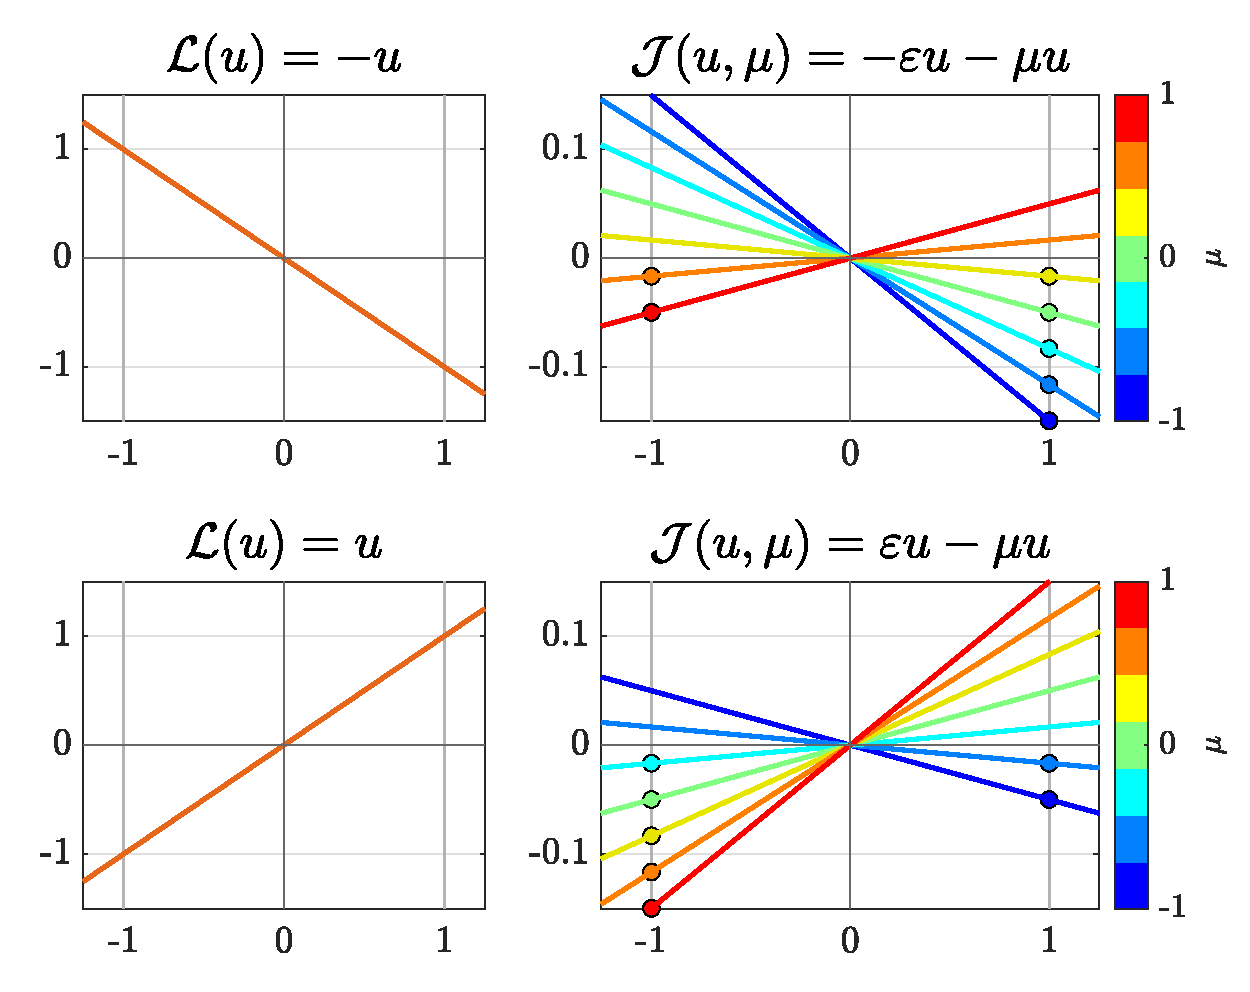
\includegraphics[scale=0.415]{img/fig03.eps}
	\caption{Bi-level SHE: in the left column we show three types of concave penalization compatibles with Theorem \ref{th:bang-bang}. In the right columns we display the behavior of the corresponding Hamiltonian for different values of $\mu$.}\label{fig:Bang-Bang-penalization} 
\end{figure}

\subsection{Proof of Theorem \ref{th:PLP}}\label{proof:PLP}

In this case, we suppose that $\mathcal{U} = \{ u_i\}_{i=1}^L$ is a finite set of real numbers in $[-1,1]$ satisfying
\begin{align*} 
	-1 = u_1 < u_2 <\ldots <u_L = 1, \quad \text{with} \ L> 2.
\end{align*} 
The case $L=2$ is just the bi-level case. As in the previous proof, we only need to show that the argmin in \eqref{eq:control design2} is a singleton and belongs to $\mathcal{U}$ for every $t\in [0,\pi]$ except for a finite number of points in $[0,\pi]$.

In this case, the study of the minimizers of $\mathcal{J}$ is slightly more involved since the penalization function $\mathcal{L}$ defined in \eqref{eq:PLP}-\eqref{eq:lambda k} is not differentiable at any point $u_k\in\mathcal U$.

Notwithstanding that, $\mathcal{L}$ is an affine interpolation of a convex function, so it is Lipschitz and convex.  Hence, $\mathcal{J}$ is also Lipschitz and convex as a function of $u$. In view of this, we know that $u$ is a minimizer of $\mathcal{J} (u,\mu)$ if and only if
\begin{equation}\label{opti cond subdiff}
	0\in \partial_u \mathcal{J} (u,\mu),
\end{equation}
where $\partial_u$ denotes the subdifferential with respect to $u$. 

Let us recall the definition of subdifferential from convex analysis:
\begin{align*}
	\partial_u \mathcal{J} (u,\mu) = \{  & c\in \mathbb{R} \quad \text{s.t.} 
	\\
	&\mathcal{J} (v,\mu) - \mathcal{J} (u,\mu) \geq c(v-u) 
	\\
	& \forall v\in [-1,1] \}. 
\end{align*}
In the case of a convex function, one may show that the subdifferential at $u\in (-1,1)$ is the nonempty interval $[a,b]$, where $a$ and $b$ are the one-sided derivatives
\begin{align*}
	a &= \lim_{v\to u^-} \frac{\mathcal{J} (v,\mu) - \mathcal{J}(u,\mu)}{v-u} 
	\\[5pt]
	b &= \lim_{v\to u^+} \frac{\mathcal{J} (v,\mu) - \mathcal{J}(u,\mu)}{v-u}. 
\end{align*}
At this regard, notice that, if $\mathcal J$ is differentiable at $u\in (-1,1)$, then the left and right derivatives coincide and we have that
\begin{align*}
	\partial_u \mathcal J(u,\mu) = \frac{d}{du} \mathcal J(u,\mu).
\end{align*}
Moreover, the subdifferential at $u=-1$ and $u=1$ are given by $(-\infty, b]$ and $[a,+\infty)$ respectively.

Using this characterization of the subdifferential, we can compute $\partial_u\mathcal{J}(u,\mu)$ for all $u\in [-1,1]$ in terms of $\mu$. To this end, let us define
\begin{align*} 
	p_k := \frac{d}{du}\lambda_k(u) = \frac{\mathcal{P}(u_{k+1}) - \mathcal{P} (u_k) }{u_{k+1} - u_k} 
\end{align*} 
for all $k\in \{1, \ldots, L-1\}$, with $\lambda_k(u)$ given by \eqref{eq:lambda k}. Using the definition of $\mathcal{J}$ in \eqref{eq:functionalJ} and $\mathcal{L}$ in \eqref{eq:PLP}, we can compute
\begin{align*}
	&\partial_u \mathcal{J} (-1,\mu) = (-\infty, \varepsilon p_1 -\mu], 
	\\[5pt]
	&\partial_u \mathcal{J} (1,\mu) = [\varepsilon p_{L-1} -\mu, +\infty), 
	\\[5pt]
	&\partial_u \mathcal{J} (u_k,\mu) = [\varepsilon p_{k-1} -\mu,  \, \varepsilon p_k -\mu],
\end{align*}
for all $k\in \{ 2, \ldots, L-1\}$, and
\begin{equation*}
	\partial_u \mathcal{J}(u,\mu) = \{\varepsilon p_k -\mu\},
\end{equation*}
for all $u\in (u_k, u_{k+1})$ and all $k\in \{ 1, \ldots, L-1 \}$.

Now we observe that
\begin{equation}\label{eq:subdiff}
	\begin{array}{ll}
		0\in \partial_u \mathcal{J} (-1,\mu) & \quad\text{iff}\quad  \mu\leq  \varepsilon p_1, 
		\\[5pt]
		0\in \partial_u \mathcal{J} (1,\mu) & \quad\text{iff} \quad \mu\geq  \varepsilon p_{L-1}, 
		\\[5pt]
		0\in \partial_u \mathcal{J} (u_k,\mu) & \quad\text{iff} \quad  \varepsilon p_{k-1} \leq \mu \leq \varepsilon p_k , 
	\end{array} 
\end{equation}
for all $k\in \{ 2, \ldots, L-1\}$,  and, for all $k\in \{ 1, \ldots, L-1 \}$,
\begin{equation}\label{eq:subdiff2}
	0\in \partial_u \mathcal{J} (u,\mu) \quad \text{for all}\  u\in [u_k, u_{k+1}]
\end{equation}
if and only if $\mu= \varepsilon p_k$.

From \eqref{eq:subdiff} and \eqref{eq:subdiff2} we immediately get that, for all $t\in[0,\pi]$,
\begin{align*}
	\argmin_{u\in[u_k,u_{k+1}]}  \mathcal{J} (u,\mu^\ast(t)) = \{u_k,u_{k+1}\}.
\end{align*}
Similarly to the bi-level case before, we then have three possible situations:
\begin{itemize}
	\item[1.] If $\mathcal{J}(u_k,\mu^\ast(t)) <  \mathcal{J}(u_{k+1},\mu^\ast(t))$, then the argmin of $\mathcal{J} (u,\mu^\ast(t))$ reduces to the singleton $\{u_k\}$.
	\vspace{0.2cm}
	\item[2.] If $\mathcal{J}(u_k,\mu^\ast(t)) >  \mathcal{J}(u_{k+1},\mu^\ast(t))$, then the argmin of $\mathcal{J} (u,\mu^\ast(t))$ reduces to the singleton $\{u_{k+1}\}$.
	\vspace{0.2cm}
	\item[3.] If $\mathcal{J}(u_k,\mu^\ast(t)) =  \mathcal{J}(u_{k+1},\mu^\ast(t))$, i.e. 
	\begin{align}\label{eq:mu_astML}
		\mu^\ast (t) = \varepsilon p_k,
	\end{align}
	then the argmin of $\mathcal{J} (u,\mu^\ast(t))$ remains the set $\{u_k,u_{k+1}\}$.
\end{itemize}

Hence, using the optimality condition \eqref{eq:control design2}, we see that $u^\ast(t)=u_k$ for some $u_k\in\mathcal U$ for all $t\in [0,\pi]$ except when $\mu^\ast(t)$ satisfies \eqref{eq:mu_astML}. In view of the form of $\mu^\ast(t)$ in \eqref{eq:m ast}, it is clear that this equality can only hold a finite number of times in the interval $[0,\pi]$. Once again, the points in $[0,\pi]$ where \eqref{eq:mu_astML} holds are precisely the switching angles.

Finally, Due to the continuity of $\mu^\ast(t)$, along with \eqref{eq:subdiff}, it is clear that $u^\ast(t)$ does not change value between two consecutive switching angles and, therefore, it possesses the staircase property of the waveform \eqref{eq:staircase prop}. \hfill $\square$

\begin{figure}[h]
	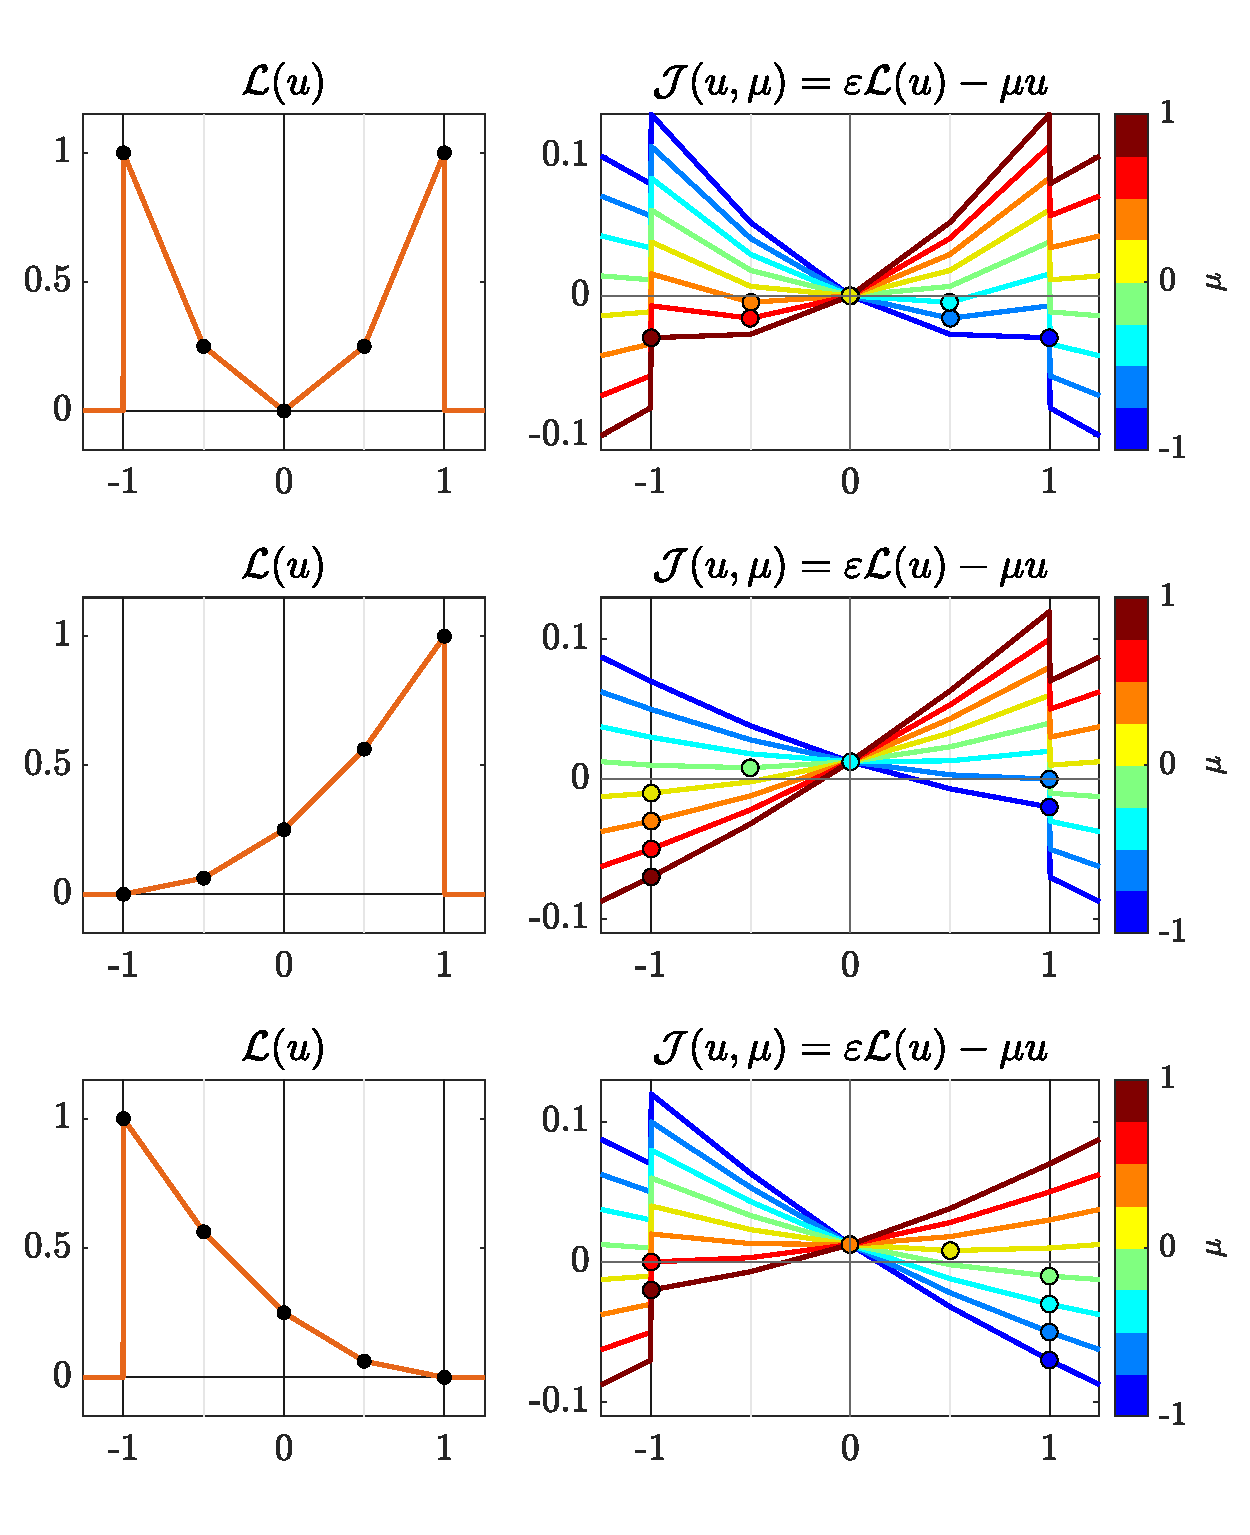
\includegraphics[scale=0.415]{img/fig04.eps}
	\caption{Multilevel SHM: in the left column we show three types of penalizations which are compatible with our theoretical results. In the right column we show the behavior of the corresponding Hamiltonian for different values of $\mu$.}\label{fig:SHE-multi}
\end{figure} 

%Hence, we have $\partial H_m = \varepsilon\partial \mathcal{L} - m$. This means that, given $m\in \mathbb{R}$, we look for $u \in [-1,1]$ minimizing $\mathcal{H}_m(u)$. It is then necessary to determine whether zero belongs to $\partial \mathcal{H}_m(u)$.
%
%\begin{itemize}
%    \item \textbf{Case 1: $m \leq \varepsilon(u_1+u_2)$}: since $m$ is less than the  minimum of all subdifferentials, then zero does not belong to any of the intervals we defined. Hence, the minimum is in one of the extrema
%    \begin{gather}
%        \argmin_{|u| < 1} \mathcal{H}_m(u) = u_1
%    \end{gather} 
%    \item \textbf{Case 2: $m = \varepsilon(u_{k+1}+u_k) $}: taking into account that $\forall k \in \{1,\dots,N_u-1\}$,
%    \begin{gather}
%        \argmin_{|u| < 1} \mathcal{H}_m(u) = [u_k,u_{k+1}[ 
%    \end{gather} 
%    \item \textbf{Case 3: $\varepsilon(u_k+u_{k-1})<m<\varepsilon(u_{k+1}+u_k)$}: taking into account that $\forall k \in \{2,\dots,N_u-1\}$,
%    \begin{gather}
%        \argmin_{|u| < 1} \mathcal{H}_m(u) = u_k
%    \end{gather}
%    \item \textbf{Case 4: $m>\varepsilon(u_{N_u}+u_{N_u-1})$}:
%    \begin{gather}
%        \argmin_{|u| < 1} \mathcal{H}_m(u) = u_{N_u}
%    \end{gather} 
%\end{itemize}
%
%In other words, only when $m = \varepsilon(u_{k+1}+u_k)$ the minima of the Hamiltonian belong to an interval. For all the other values of $m\in\mathbb{R}$, these minima are contained in $\mathcal{U}$. So that under a continuous variation of $m$, Case 2 can only occur pointwise. Recalling the optimal control problem $m(\tau) = [\bm{p}(\tau) \cdot \bm{\mathcal{D}}(\tau)]$, we can notice that Case 2 corresponds to the instants $\tau$ of change of value.

\section{Conclusions}\label{sec:conclusions}

In this paper, we have considered the Selective Harmonic Modulation problem, consisting in generating a staircase control signal $u$ with a desired harmonic spectrum, and we have proposed a novel optimal control-based approach to solve it. In more detail, we have shown how the SHM Problem \eqref{pb:SHEp} can be cast as a null-controllability one for a dynamical system describing the evolution in the interval $[0,\pi)$ of the Fourier coefficients of $u$, which plays the role of a control for this dynamics. In this framework, $u$ can then be obtained through the minimization of a suitable penalized cost functional. Moreover, by choosing properly the penalization term, the staircase form of $u$ can be guaranteed without imposing further restrictions in the optimization process.

One of the main advantages of our methodology with respect to the previously existing ones is that, tackling SHM under the perspective of optimal control, we are able to solve several critical issues (described in detail in Section \ref{sec:SHE_finite-dim_pbm}) arising in practical applications. Therefore, our approach yields important advantages for the SHM community and settles solid basis for future developments in this field.

This work provides an exhaustive analysis of the SHM problem under the perspective of optimal control. Notwithstanding that, some relevant issues have not been completely covered by our study, and will be considered in future works:
\begin{itemize}
	\item[1.] Continuity problem.
	\item[2.] Estimate of the error (with respect to $\theta$) when regularizing $\mathcal L$.
	\item[3.] Solving numerically SHM without regularizing $\mathcal L$.
\end{itemize}

\begin{ack}            
This project has received funding from the European Research Council (ERC) under the European Union’s Horizon 2020 research and innovation programme (grant agreement NO: 694126-DyCon). The work of U.B. and J.O. is partially supported by the Elkartek grant KK-2020/00091 CONVADP of the Basque government. The work of U.B. is partially supported by the Air Force Office of Scientific Research (AFOSR) under Award NO: FA9550-18-1-0242 and by the Grant MTM2017-92996-C2-1-R COSNET of MINECO (Spain).
\end{ack}
 
\bibliographystyle{apalike}        % Include this if you use bibtex 
\bibliography{bib}           % and a bib file to produce the 
                                 % bibliography (preferred). The
                                 % correct style is generated by
                                 % Elsevier at the time of printing.


 

\end{document} 